%%% Hlavní soubor. Zde se definují základní parametry a odkazuje se na ostatní části. %%%

%% Verze pro jednostranný tisk:
% Okraje: levý 40mm, pravý 25mm, horní a dolní 25mm
% (ale pozor, LaTeX si sám přidává 1in)
%\documentclass[12pt,a4paper]{report}
%\setlength\textwidth{145mm}
%\setlength\textheight{247mm}
%\setlength\oddsidemargin{15mm}
%\setlength\evensidemargin{15mm}
%\setlength\topmargin{0mm}
%\setlength\headsep{0mm}
%\setlength\headheight{0mm}
% \openright zařídí, aby následující text začínal na pravé straně knihy
%\let\openright=\clearpage

%% Pokud tiskneme oboustranně:
\documentclass[12pt,a4paper,twoside,openright]{book}
\setlength\textwidth{145mm}
%\setlength\textheight{247mm}
\setlength\oddsidemargin{15mm}
\setlength\evensidemargin{0mm}
%\setlength\topmargin{0mm}
%\setlength\headsep{0mm}
%\setlength\headheight{0mm}
\let\openright=\cleardoublepage

%% Ostatní balíčky
\usepackage{graphicx}
\usepackage{amsfonts, amsmath, amsthm, amssymb}
\usepackage[T1]{fontenc}
\usepackage[utf8]{inputenc}
\usepackage[english]{babel}
\usepackage[all,cmtip]{xy}
\usepackage{textcomp}
\usepackage{subfloat}
\usepackage{graphicx}
\usepackage{lmodern}
\usepackage{microtype}
\usepackage[utf8]{inputenc}
\usepackage{booktabs}
\usepackage{a4wide}
\usepackage{comment}
\usepackage{array}
\usepackage[lofdepth,lotdepth]{subfig}
%\usepackage{natbib}
\usepackage{tgpagella}
%\usepackage{tgcursor}
\usepackage{tikz}
\usetikzlibrary{decorations.pathreplacing,patterns}

\usepackage{listings}
\lstloadlanguages{Haskell}
\lstnewenvironment{code}
    {\lstset{}%
      \csname lst@SetFirstLabel\endcsname}
    {\csname lst@SaveFirstLabel\endcsname}
    \lstset{
      comment=[l]--,
      basicstyle=\small\sffamily,
      keywordstyle=\bf\sffamily,
      commentstyle=\color{gray}\it\rmfamily,
      columns=fullflexible,
      basewidth={0.5em,0.45em},
      xleftmargin=2em,
      morekeywords={data,where},
      literate=
      	{+}{{$+$}}1
      	{/}{{$/$}}1
      	{*}{{$*$}}1
      	{=}{{$=$}}1
        {>}{{$>$}}1
        {<}{{$<$}}1
        {\\}{{$\lambda$}}1
        {\\\\}{{\char`\\\char`\\}}1
       	{->}{{$\rightarrow\:$}}2
       	{>=}{{$\geq$}}2
       	{<-}{{$\leftarrow$}}2
        {<=}{{$\leq$}}2
        {=>}{{$\Rightarrow$}}2 
        {\ .}{{$\circ$}}2
        {\ .\ }{{$\circ$}}2
        {>>}{{>>}}2
        {>>=}{{>>=}}2
        {|}{{$\mid$}}1
        {Nat}{{$\mathbb{N}\:$}}1
        {forall}{{$\forall\:$}}1
    }

%\usepackage{minion}
%\renewcommand{\scdefault}{ssc}
%\newfont{\chapnum}{eurb10 scaled 10000}
%\newcommand{\lowercaps}[1]{\textsc{\MakeLowercase{#1}}}
%\newcommand{\uppercaps}[1]{\textsc{\MakeUppercase{#1}}}

%% Balíček hyperref, kterým jdou vyrábět klikací odkazy v PDF,
%% ale hlavně ho používáme k uložení metadat do PDF (včetně obsahu).
%% POZOR, nezapomeňte vyplnit jméno práce a autora.
\usepackage{color}
\definecolor{link}{rgb}{0,0,0.5}
\usepackage[
	colorlinks=true,
	linkcolor=link,
	urlcolor=link,
	citecolor=link,
	unicode
]{hyperref}
\hypersetup{pdftitle=On the semantics of exceptions for high level and low level languages}
\hypersetup{pdfauthor=Matus Tejiscak}

%%% Drobné úpravy stylu

% Tato makra přesvědčují mírně ošklivým trikem LaTeX, aby hlavičky kapitol
% sázel příčetněji a nevynechával nad nimi spoustu místa. Směle ignorujte.
%\makeatletter
%\def\@makechapterhead#1{
%  {\parindent \z@ \raggedright \normalfont
%   \Huge\bfseries \thechapter. #1
%   \par\nobreak
%   \vskip 20\p@
%}}
%\def\@makeschapterhead#1{
%  {\parindent \z@ \raggedright \normalfont
%   \Huge\bfseries #1
%   \par\nobreak
%   \vskip 20\p@
%}}
%\makeatother

% Toto makro definuje kapitolu, která není očíslovaná, ale je uvedena v obsahu.
\def\chapwithtoc#1{
\chapter*{#1}
\addcontentsline{toc}{chapter}{#1}
}

\title{On the semantics of exceptions for high level and low level languages}
\author{Matúš Tejiščák}

\begin{document}

\frontmatter

% Trochu volnější nastavení dělení slov, než je default.
\lefthyphenmin=2
\righthyphenmin=2

%%% Titulní strana práce

\pagestyle{empty}
\begin{center}

\large

Charles University in Prague

\medskip

Faculty of Mathematics and Physics

\vfill

{\bf\Large MASTER THESIS}

\vfill

\centerline{\mbox{
\includegraphics[width=60mm]{figures/logo}}}

\vfill
\vspace{5mm}

{\LARGE Matúš Tejiščák}

\vspace{15mm}

% Název práce přesně podle zadání
{\LARGE\bfseries On the semantics of exceptions for high level and low level languages}

\vfill

% Název katedry nebo ústavu, kde byla práce oficiálně zadána
% (dle Organizační struktury MFF UK)
Department of Theoretical Computer Science and Mathematical Logic

\vfill

\begin{tabular}{rl}

Supervisor of the master thesis: & Wouter Swierstra PhD\\
\noalign{\vspace{2mm}}
Study programme: & Computer science \\
\noalign{\vspace{2mm}}
Specialization: & Theoretical computer science \\
\end{tabular}

\vfill

% Zde doplňte rok
Prague 2012

\end{center}

\newpage

%%% Následuje vevázaný list -- kopie podepsaného "Zadání diplomové práce".
%%% Toto zadání NENÍ součástí elektronické verze práce, nescanovat.

%%% Na tomto místě mohou být napsána případná poděkování (vedoucímu práce,
%%% konzultantovi, tomu, kdo zapůjčil software, literaturu apod.)

\openright

\noindent
Dedication. % TODO

\newpage

%%% Strana s čestným prohlášením k diplomové práci

\vglue 0pt plus 1fill

\noindent
I declare that I carried out this master thesis independently, and only with the cited
sources, literature and other professional sources.

\medskip\noindent
I understand that my work relates to the rights and obligations under the Act No.
121/2000 Coll., the Copyright Act, as amended, in particular the fact that the Charles
University in Prague has the right to conclude a license agreement on the use of this
work as a school work pursuant to Section 60 paragraph 1 of the Copyright Act.

\vspace{10mm}

\hbox{\hbox to 0.5\hsize{%
In Prague, date .....................
\hss}\hbox to 0.5\hsize{%
signature of the author
\hss}}

\vspace{20mm}
\newpage

%%% Povinná informační strana diplomové práce

\vbox to 0.5\vsize{
\setlength\parindent{0mm}
\setlength\parskip{5mm}

Název práce:
On the semantics of exceptions for high level and low level languages
% přesně dle zadání

Autor:
Matúš Tejiščák

Katedra:  % Případně Ústav:
Katedra teoretické informatiky a matematické logiky
% dle Organizační struktury MFF UK

Vedoucí diplomové práce:
Wouter Swierstra PhD, Software Technology Group of Utrecht University
% dle Organizační struktury MFF UK, případně plný název pracoviště mimo MFF UK

Abstrakt:
TODO
% abstrakt v rozsahu 80-200 slov; nejedná se však o opis zadání diplomové práce

Klíčová slova:
závisle typované programování, výjimky, kompilátor, korektnost
% 3 až 5 klíčových slov

\vss}\nobreak\vbox to 0.49\vsize{
\setlength\parindent{0mm}
\setlength\parskip{5mm}

Title:
On the semantics of exceptions for high level and low level languages
% přesný překlad názvu práce v angličtině

Author:
Matúš Tejiščák

Department:
Department of Theoretical Computer Science and Mathematical Logic
% dle Organizační struktury MFF UK v angličtině

Supervisor:
Wouter Swierstra PhD, Software Technology Group of Utrecht University
% dle Organizační struktury MFF UK, případně plný název pracoviště
% mimo MFF UK v angličtině

Abstract:
TODO
% abstrakt v rozsahu 80-200 slov v angličtině; nejedná se však o překlad
% zadání diplomové práce

Keywords:
dependently-typed programming, exceptions, compiler, correctness
% 3 až 5 klíčových slov v angličtině

\vss}

\newpage

%%% Strana s automaticky generovaným obsahem diplomové práce. U matematických
%%% prací je přípustné, aby seznam tabulek a zkratek, existují-li, byl umístěn
%%% na začátku práce, místo na jejím konci.

\openright
\pagestyle{plain}
\setcounter{page}{1}
\tableofcontents

%%% Jednotlivé kapitoly práce jsou pro přehlednost uloženy v samostatných souborech
\mainmatter
\chapter*{Introduction}
\addcontentsline{toc}{chapter}{Introduction}

% SPJ says:
% 1. Describe the problem
% 2. State your contributions
% ...and that's all.

This thesis deals with the semantics of exceptions in programming languages and how the semantics
is preserved by the compilation process.

To verify a~compiler that compiles code from a~high-level language (such as Haskell)
to a~low-level language (such as the x86 assembler), we need (besides other things):
\begin{itemize}
	\item to \emph{state semantics} and properties of the \emph{high-level} language;
	\item to \emph{state semantics} for \emph{low-level} code that results from the compilation process;
	\item to \emph{prove} that compilation preserves this semantics;
	\item to \emph{formalize} the above three points in a~way that allows for mechanical verification.
\end{itemize}
Clearly, without these ingredients, there is no way to define what correctness of a~compiler actually
means (let alone prove it).

In this thesis, we pursue the above four goals, focused on a simple language with exceptions.
Besides these core objectives, we want our solution to have other properties, all related
to being useful in practical compiler development:

\begin{itemize}\label{objectives}

	\item the specifications should be \emph{runnable}; that is, the result should be a~program
		that can be run, that can provide compiled code for given input code fragments, and
		that can execute the compiled code, producing actual results;
		
	\item the program should be \emph{readable}. Even though the program may be verified,
		it should still convey the mechanism of execution clearly without proof clutter getting
		in the way of comprehension;
		
	\item the compiled code should be \emph{executable by a~simple machine} (a~stack machine,
		for instance), with fully explicit state and no fancy high-level features such as
		continuations, arbitrarily-sized instructions or implicit stacks;
		
	\item there should be an~obvious and \emph{straightforward way to extract} the executable core
		sans proofs into other (mainstream) languages, either manually or automatically,
		for practical use.
		
\end{itemize}

\noindent The contributions of this thesis are:
\begin{itemize}
	\item We formalize the discussed semantics for a~simple language of expressions
		featuring binary operators\footnote{We actually implement only addition but adding new
		operators is trivial.} and exceptions, using the language as our high-level language
		(Section \ref{sec:expression-semantics});
	\item we explore approaches to the design of execution of low-level code on a~virtual
		machine, first examining an approach found in the
		literature, then presenting a~modified one that is easier to implement in a~dependent
		setting by gradually improving on a naive solution and explaining the choices
		(Sections \ref{sec:own-execution-gmh} to \ref{sec:linearized-code});
	\item we formalize the semantics of a~language of instructions for a~simple stack machine,
		which is our target low-level language, using the latter approach
		(Section \ref{sec:lin-instr-semantics});
	\item we define a~compiler generating instruction sequences from expressions in the high-level
		language (Section \ref{sec:lin-compile});
	\item we prove that the semantics is preserved in code generated by this compiler
		(Section \ref{sec:lin-correctness}).
\end{itemize}

\noindent We use the general-purpose dependently typed pure functional language Agda in
our development.
Readers of this thesis are assumed to have knowledge of functional programming, but
not necessarily dependently typed programming. A~brief introduction to dependent types and
related concepts for the purposes of this thesis will be given in Chapter \ref{chap:dependent-types}.

\pagestyle{headings}
\chapter{Exceptions in programming languages}

``Exceptions'' is a broader term referring to a strategy of handling erroneous
states in computer programs by interrupting normal program execution, running special
code called an \emph{exception handler} and then resuming execution in a known, different
state.

The usual terminology is not very strict: the word ``exception'' may mean sligtly
different things -- or different sides of the same thing -- in different contexts.
For example, programming languages are said to \emph{have exceptions} if they support
this kind of error handling; exceptions are said to \emph{be compiled}, while it is the
corresponding infrastructure and support code that is compiled; often the word ``exception''
denotes a piece of information about the error being handled; et cetera.

When an error occurs during normal execution of a program, \emph{an exception is thrown}%
\footnote{Some programming languages, such as Python, use the term \emph{raised}.%
\cite{python:reference}}.
This starts the
process of \emph{handling the exception}: looking for a suitable
\emph{exception handler} that \emph{handles the exception}, either by \emph{catching} it
to resume normal computation, or by \emph{re-throwing} it to find another handler
able to deal with the error.

Due to common names of the corresponding syntactic features of popular programming languages%
\footnote{Most of them use the same keywords for this purpose.},
a piece of code together with attached pieces of handler code is called a \emph{try-block},
and a piece of handler code is called a \emph{catch-block}.

Most languages also provide \emph{finally-blocks}. These are pieces of code attached to a
try-block that are guaranteed to be executed after the try-block, whether an exception
has been thrown or not. Because of this property, finally-blocks are usually used to clean up
resources. In this thesis, we will not model finally-blocks as these can be
supplemented by an appropriate use of all-catching exception handlers.

There may be multiple handlers attached to a piece of code.
As already mentioned, the word ``exception'' also denotes a piece of information about
the error or condition causing the exceptional state, modeled by a value of the programming
language. In typed languages, these values have types, exception handlers declare what
types of exceptions they can handle, and based on the type of the thrown exception,
an appropriate handler is selected. The handler can then inspect the exception and
behave appropriately.

A try-block needn't have handlers for all exceptions that might arise within. If an exception
is \emph{uncaught} within a try-block, it is \emph{propagated} to the containing try-block,
which may not catch this exception as well, propagating it further.
If an exception propagates all the way out of all nested try-blocks, the program usually
aborts.

To give a quick illustration how try-blocks look in the concrete syntax of some widely used
languages, \Fref{fig:try-blocks} contains four examples.\footnote{Note that OCaml does not
have syntax for finally-blocks; these are simulated by a function. Haskell does not have
syntax for exceptions at all, both \emph{catch} and \emph{finally} are just functions.
All code snippets are just symbolic and have been stripped of non-relevant context, such
as library imports and the definitions of the functions \emph{perform\_work}
and \emph{do\_cleanup}.}

\begin{figure}
%
\begin{subfigure}[b]{0.46\textwidth}\begin{codepy}
try:
	perform_work()
except IOError:
	print "IO error caught"
finally:
	do_cleanup()
\end{codepy}\caption{Python}\end{subfigure}
%
\begin{subfigure}[b]{0.46\textwidth}\begin{codejava}
try {
	performWork();
} catch (IOException e) {
	System.out.println(
	    "IO error caught");
} finally {
	doCleanup();
}
\end{codejava}\caption{Java}\end{subfigure}

\begin{subfigure}[b]{0.46\textwidth}\begin{codehs}
performWork
 `catch` (\(e :: IOException) ->
   putStrLn "IO error caught")
 `finally` 
   doCleanup
\end{codehs}\caption{Haskell}\end{subfigure}
%
\begin{subfigure}[b]{0.46\textwidth}\begin{codeml}
finally do_cleanup (fun () ->
  try perform_work ()
  with IO_error ->
    print_string "IO error caught"
) ()
\end{codeml}\caption{OCaml}\end{subfigure}

\caption{Try-blocks in different languages}
\label{fig:try-blocks}
\end{figure}

\todo{Really include ``finally''? Revise OCaml.}

\section{Purpose}

As already mentioned, in practice, exceptions are mostly used to handle errors or
other exceptional states. The advantage to using
exceptions for this purpose is separation of concerns and hence cleaner resulting code.
Especially when reading a program, the reader first reads the code related the expected
execution path, uncluttered with error checks, which brings forward the main idea
of the code.

However, some languages, for example Python or OCaml, use exceptions also for control-flow
purposes, not only in rare critical events. Python iterators raise an exception to
indicate the end of stream \cite{python:reference}; also file-I/O functions in OCaml raise
an exception to indicate the end of file \cite{ocaml:reference}. The implementation of
exceptions in these languages is efficient enough to make them cheap and enable this approach.

\todo{Disadvantages. Multiple exit points, reasoning.}

\todo{Extend this section.}

\section{History}

Louden and Lambert describe the invention of exceptions in their book
\emph{Programming Languages: Principles and Practice} as follows.

\begin{quote}
Exception handling was pioneered by the language PL/I in the 1960s and
significantly advanced by CLU in the 1970s, with the major design questions
eventually resolved in the 1980s and early 1990s. Today, virtually all major
current languages, including C++, Java, Ada, Python, ML, and Common Lisp (but
not C, Scheme or Smalltalk) have built-in exception handling mechanisms.
Exception handling has, in particular, been integrated very well into
object-oriented mechanisms in Python, Java, and C++, and into functional
mechanisms in ML and Common Lisp. Also, languages that do not have built-in
mechanisms sometimes have libraries available that provide them, or have other
built-in ways of simulating them. \cite[p.~423]{louden:languages}
\end{quote}

% http://stackoverflow.com/questions/1449951/what-language-was-the-first-to-implement-exception-handling

\todo{Extend this section.}

\section{Theoretical appeal}

The theoretical appeal of exceptions in function languages is impossible to discuss
without having introduced the \emph{Curry-Howard correspondence}.

\subsection{The Curry-Howard correspondence}

The Curry-Howard correspondence establishes a relationship between typed programs and logic.
According to this interpretation, types of programs correspond to logical propositions --
and programs themselves correspond to proofs of logical propositions corresponding to their
types.

This correspondence goes all the way to relating whole $\lambda$-calculi to different
logical systems. For example, the simply typed $\lambda$-calculus corresponds to the minimal
logic, see \Fref{fig:stlc-ml}.

\begin{figure}
\centering
\begin{subfigure}[b]{0.45\textwidth}
\begin{prooftree}
\bax{$x : \sigma \in \Gamma$}
\bright{Ax}\bun{$\Gamma \vdash x : \sigma$}
\end{prooftree}
\begin{prooftree}
\bax{$\Gamma, x : \sigma \vdash M : \tau$}
\bright{Abstr}\bun{$\Gamma \vdash (\lambda x:\sigma. M) : \sigma \to \tau$}
\end{prooftree}
\begin{prooftree}
\bax{$\Gamma \vdash f : \sigma \to \tau$}
\bax{$\Gamma \vdash x : \sigma$}
\bright{App}\bbin{$\Gamma \vdash f x : \tau$}
\end{prooftree}

\caption{$\lambda_\to$}
\end{subfigure}
%
\begin{subfigure}[b]{0.45\textwidth}
\begin{prooftree}
\bax{$A \in \Gamma$}
\bright{Ax}\bun{$\Gamma \vdash A$}
\end{prooftree}
\begin{prooftree}
\bax{$\Gamma, A \vdash B$}
\bright{$I_\to$}\bun{$\Gamma \vdash A \to B$}
\end{prooftree}
\begin{prooftree}
\bax{$\Gamma \vdash A \to B$}
\bax{$\Gamma \vdash A$}
\bright{$E_\to$}\bbin{$\Gamma \vdash B$}
\end{prooftree}
\caption{$ML$}
\end{subfigure}

\caption{Simply typed $\lambda$-calculus ($\lambda_\to$), compared to minimal logic (ML).}
\label{fig:stlc-ml}
\end{figure}

When put side-by-side, it can be seen that the typing rules for the simply typed
$\lambda$-calculus become precisely the natural-deduction rules for minimal logic
if terms are erased and only types are retained.

In this interpretation, \emph{function application} on the computational side corresponds
to \emph{modus ponens} (or implication elimination) on the logic side, and
\emph{$\lambda$-abstraction} corresponds to the \emph{deduction theorem} (or implication
introduction).

The correspondence between certain $\lambda$-calculi and logic systems was presented
by Barendregt in \cite{barendregt91} in the elegant form of the $\lambda$-cube, as seen in
\Fref{fig:lambda-cube}. The names of the $\lambda$-calculi and the corresponding
logic systems are listed in \Fref{tab:lambda-cube}.

\begin{figure}
\centering
\begin{subfigure}{0.4\textwidth}
\begin{tikzpicture}[x=9mm,y=9mm,
        back line/.style={densely dotted,-},
        normal line/.style={-stealth,-},
        cross line/.style={normal line,-,
           preaction={draw=white, -, 
           line width=6pt}},
    ]
    \draw
    	(0,0) node{$\lambda_\to$}
    	(3,0) node{$\lambda{}P$}
    	(0,3) node{$\lambda{}2$}
    	(3,3) node{$\lambda{}P2$}
    	(1,1) node{$\lambda\underline{\omega}$}
    	(4,1) node{$\lambda{}P\underline{\omega}$}
    	(1,4) node{$\lambda\omega$}
    	(4,4) node{$\lambda{}C$}
	    ;
	\draw
		(1,1)
		+(0.5,0) edge[back line] +(2.5,0)
		+(0,0.5) edge[back line] +(0,2.5)
		+(0.5,3) edge[normal line] +(2.5,3)
		+(3,0.5) edge[normal line] +(3,2.5)
		;
	\draw[normal line]
		(0,0)
		+(0.5,0) edge +(2.5,0)
		+(0,0.5) edge +(0,2.5)
		+(0.5,3) edge[cross line] +(2.5,3)
		+(3,0.5) edge[cross line] +(3,2.5)
		;
	\draw
		(0,3) +(0.25,0.25) edge[normal line] +(0.7,0.7)
		(3,3) +(0.25,0.25) edge[normal line] +(0.7,0.7)
		(3,0) +(0.25,0.25) edge[normal line] +(0.7,0.7)
		(0,0) +(0.25,0.25) edge[back line] +(0.7,0.7)
		;
\end{tikzpicture}
\caption{$\lambda$-cube}
\end{subfigure}
%
\begin{subfigure}{0.4\textwidth}
\begin{tikzpicture}[x=9mm,y=9mm,
        back line/.style={densely dotted,-},
        normal line/.style={-stealth,-},
        cross line/.style={normal line,-,
           preaction={draw=white, -, 
           line width=6pt}},
    ]
    \draw[font=\footnotesize]
    	(0,0) node{PROP}
    	(3,0) node{PRED}
    	(0,3) node{PROP2}
    	(3,3) node{PRED2}
    	(1,1) node{PROP$\underline{\omega}$}
    	(4,1) node{PRED$\underline{\omega}$}
    	(1,4) node{PROP$\omega$}
    	(4,4) node{PRED$\omega$}
	    ;
	\draw
		(1,1)
		+(0.8,0) edge[back line] +(2.2,0)
		+(0,0.3) edge[back line] +(0,2.7)
		+(0.8,3) edge[normal line] +(2.2,3)
		+(3,0.3) edge[normal line] +(3,2.7)
		;
	\draw[normal line]
		(0,0)
		+(0.8,0  ) edge +(2.2,0  )
		+(0  ,0.3) edge +(0  ,2.7)
		+(0.8,3  ) edge[cross line] +(2.2,3  )
		+(3  ,0.3) edge[cross line] +(3  ,2.7)
		;
	\draw
		(0,3) +(0.25,0.25) edge[normal line] +(0.7,0.7)
		(3,3) +(0.25,0.25) edge[normal line] +(0.7,0.7)
		(3,0) +(0.25,0.25) edge[normal line] +(0.7,0.7)
		(0,0) +(0.25,0.25) edge[back line] +(0.7,0.7)
		;
\end{tikzpicture}
\caption{Logic-cube}
\end{subfigure}
%
\caption{The $\lambda$-cube and the corresponding logic-cube \cite{barendregt91}}
\label{fig:lambda-cube}
\end{figure}

\begin{table}
\centering
\begin{tabular}{lll}
\toprule
\textit{$\lambda$-calculus} & \textit{logic} & \textit{description} \\
\midrule
$\lambda_\to$ & PROP & first-order propositional \\
$\lambda{}P$ & PRED & first-order predicate \\
$\lambda{}2$ & PROP2 & second-order propositional \\
$\lambda{}P2$ & PRED2 & second-order predicate \\
$\lambda\underline{\omega}$ & PROP$\underline{\omega}$ & weakly higher-order propositional \\
$\lambda{}P\underline{\omega}$& PRED$\underline{\omega}$ & weakly higher-order predicate \\
$\lambda\omega$ & PROP$\omega$ & higher-order propositional \\
$\lambda{}C$ & PRED$\omega$ & higher-order predicate \\
\bottomrule
\end{tabular}

\vspace{8pt}
{\small The calculus $\lambda_\to$ is also called the \emph{simply typed $\lambda$-calculus} (STLC)
and the calculus $\lambda{}C$ is also called the \emph{calculus of constructions} (CoC).}
\caption{The $\lambda$-calculi and logic systems of the $\lambda$-cube \cite{barendregt91}}
\label{tab:lambda-cube}
\end{table}

\todo{Talk about dependent types, Coq, proving, Type theory, \ldots ?}

\subsection{Control operators}

In functional languages, exceptions are closely related to the theory of
\emph{control operators}\footnote{Such as \ident{call/cc} in Scheme.},
for example the calculus $\lC$ introduced by Felleisen in \cite{felleisen87}
as a way to reason about abortive programs. An accessible formal description
thereof can be found in \cite[p.~876, Section~3]{ariola-herbelin} or
\cite{griffin90}; here we will restrict ourselves to an informal sketch.

Felleisen introduced three control operators, $\bigC$ for ``control'', $\bigA$
for ``abort'', and $\bigK$ for \ident{call/cc}. The operator $\bigA$
takes a value and replaces the current context with it; the operator $\bigK$
takes a function and applies it to the current context (reified as a continuation),
and finally the operator $\bigC$ takes a function and replaces the current context
with the function applied to the original context, thus being a combination of
the former two; an overview can be seen in \Fref{tab:control-operators}.

\begin{table}
\centering
\begin{tabular}{llll}
\toprule
\thead{Operator} & \thead{Replaces CC*} & \thead{Provides CC**} & \thead{In terms of the others} \\
\midrule
$\bigC$ & yes & yes & $\lambda M.\,\bigK(\lambda k.\,\bigA (M k))$\\
$\bigK$ & no***	& yes & $\lambda M.\,\bigC(\lambda k.\,k (M k)) $ \\
$\bigA$ & yes & no & $\lambda M.\,\bigC(\lambda \_.\,M)$ \\
\bottomrule
\end{tabular}

\vspace{2pt}
{\footnotesize *Current context. **Applies its argument to the current continuation.
***Context replacement happens only when (if ever) the provided continuation is applied.}
\caption{Overview of control operators}
\label{tab:control-operators}
\end{table}

The behavior of these operators is best shown on an example. The simplest one is the abort
operator $\bigA$. Let $E$ be some $\lambda$-context. Then the operator $\bigA$ reduces
as follows.
\begin{equation*}
	E[\bigA(M)] \red M
\end{equation*}
For example:
\begin{equation*}
	1 + (2 \cdot \bigA(3)) \red 3
\end{equation*}
No matter what the context is, all of it is replaced by the argument to $\bigA$. Hence,
the operator $\bigA$ provides ``escape'' to the top-level. Note that any computation commenced
(here, adding the $1$ and multiplying by $2$) is discarded and evaluation starts anew
with whatever $\bigA$ took as the argument.

\begin{figure}
\centering
\begin{subfigure}[t]{0.4\textwidth}
\begin{eqnarray*}
&&2 \cdot (3 + \underline{\bigC(\lambda k.\, 4 + k\, 5)}) \\
&&{} \red 2 \cdot (3 + \underline{5}) \\
&&{} \red 16
\end{eqnarray*}
\caption{Throwing to $\bigC$}\label{fig:CK-throwC}
\end{subfigure}
%
\begin{subfigure}[t]{0.4\textwidth}
\begin{eqnarray*}
& 2 \cdot (3 + \underline{\bigK(\lambda k.\, 4 + k\, 5)}) \\
& {} \red 2 \cdot (3 + \underline{5}) \\
& {} \red 16
\end{eqnarray*}
\caption{Throwing to $\bigK$}\label{fig:CK-throwK}
\end{subfigure}

\begin{subfigure}[t]{0.4\textwidth}
\begin{eqnarray*}
& 2 \cdot (3 + \bigC(\lambda \_.\, \underline{4 + 5})) \\
& {} \red \underline{4 + 5} \\
& {} \red 9
\end{eqnarray*}
\caption{Not throwing to $\bigC$}\label{fig:CK-nothrowC}
\end{subfigure}
%
\begin{subfigure}[t]{0.4\textwidth}
\begin{eqnarray*}
& 2 \cdot (3 + \bigK(\lambda \_.\, \underline{4 + 5})) \\
& {} \red 2 \cdot (3 + \underline{9}) \\
& {} \red 24
\end{eqnarray*}
\caption{Not throwing to $\bigK$}\label{fig:CK-nothrowK}
\end{subfigure}

\caption{Examples of reduction with $\bigC$ and $\bigK$}
\label{fig:CK}
\end{figure}

Now let us describe the operators $\bigC$ and $\bigK$ in \Fref{fig:CK}. Both of
them are similar in that the function passed
as the argument to either of the two operators takes one argument $k$, which represents
the context at the point of application of the control operator. In the case described
in Figure \ref{fig:CK}, the context
looks like $2 \cdot (3 + \square)$, the $\square$ being a hole placed exactly where
the control operator was located.

The argument $k$ is a continuation and it can be applied like a function -- except that it
is \emph{not} a function since applying it to an argument $x$ replaces the whole evaluation
context by the context represented by $k$, having the hole filled with the value $x$.
This happens in Figure \ref{fig:CK-throwC} and \Fref{fig:CK-throwK}.

In other words, applying the continuation $k$ to a value makes seemingly the control operator
``return'' that value immediately, much like a \ident{return} statement in functions in procedural
languages.

Application of the continuation $k$ to an argument is usually described as
\emph{throwing} to the continuation.

The difference between $\bigC$ and $\bigK$ shows when the function being their argument
\emph{does not throw} to the continuation and instead returns a value normally. In that case,
the operator $\bigC$ \emph{aborts} and replaces the whole evaluation context with the returned
value -- unlike the operator $\bigK$, that simply returns the value without manipulating
the context.

This can be seen in Figure \ref{fig:CK-nothrowC} and \Fref{fig:CK-nothrowK}, where the
computation $4 + 5$ either replaces the whole context ($\bigC$) or is simply returned
($\bigK$).\footnote{Apparently, here we use the call-by-name evaluation strategy, which
is arguably more suitable for demonstrational purposes. The $\lC$ calculus however comes
also in the call-by-value flavor, which is in fact the variant that fits Scheme.}

\subsubsection{Control operators and Curry-Howard}

In 1990, Griffin showed \cite{griffin90} that the control operator $\mathcal{C}$
used in $\lC$ can be given the type $\neg \neg A \to A$, yielding a \emph{computational
interpretation} of classical logic. However, this calculus did not match
classical natural deduction operationally \cite{ariola-herbelin}.

\todo{$\bigA$ is EFQ, $\bigC$ is DN, $\bigK$ is PL. DN implies everything ($\bigC$
subsumes the other two) and EFQ+PL implies DN (as $\bigC$ is definable from $\bigA$
and $\bigK$).}

From the other direction, Parigot created the $\lambda_\mu$ calculus \cite{parigot92}
as a way to assign computational content to classical natural deduction. The calculus
$\lambda_\mu$ Parigot presented did not readily correspond to classical logic --
only to minimal classical logic -- but it
can be extended to do so, finally yielding a calculus matching classical natural deduction
\cite{ariola-herbelin}.

\todo{Hence, control operators extend our logic up to classical logic!}

\subsection{Exceptions and control operators}

\todo{(Statically-bounded) exceptions can be implemented using control operators.}

\todo{Not the same, dynamic vs. static scoping \cite{thielecke:contrast, kameyama:dynamic}.}

\todo{With fresh variables, Peirce can be done.}

\section{Practical appeal}

\todo{Appeal of certified compilers.}

\label{chap:dependent-types}







































































\chapter{Dependently typed programming in Agda}
\label{chap:dependent-types}

We will create our development in a dependently typed pure functional language named Agda.
This chapter provides a (very) brief introduction to Agda, along with some commentary about
related topics.

%\todo{...and also presents reasons why Agda was chosen as the implementation language. Does it present the reasons?}

The aim is to provide the bare necessities for reading this thesis if the reader is not
familiar with Agda or dependently typed programming -- it is mostly an overview of Agda syntax
and some basic techniques used.

%\todo{Not only language but also logic. Per Martin-L\"{o}f's Type Theory? Dependent types. 
%The Curry-Howard correspondence. Total functional programming.
%Structural recursion and termination. Formal verification. The Agda proof assistant.}

For a much more complete introduction to Agda and dependently typed programming, see the
tutorial by Norell \cite{norell08} or any other tutorial from the Agda wiki \cite{agda-wiki}.

\section{A simple exceptionless language}
\label{sec:simple-language}

As a brief Agda crash-course, we will implement a very simple compiler for
a~language of arithmetical expressions to instructions for a stack machine.

Being a simple and instructive task, this has been done many times in a variety
of programming languages in other papers, publications, blog posts, et cetera;
for example in Epigram \cite{epigram-compiler} or in Coq \cite{chlipala:compiler}.

All high-level languages in this thesis will be languages of simple, typed
expressions and our first language will feature only natural numbers, addition,
and no exceptions. Besides demonstrating how dependent programming in Agda
looks like, we will also implement the auxiliary ecosystem of the
compiler and the skeleton of our development, upon which we will build later
throughout the thesis.

\todo{Add a reference to the source code.}

% branch: no-exceptions

\subsection{Type universe}

It is probably reasonable to expect a programming language to be able to represent
expressions of different types (e.g. Integer or Boolean).

Hence the first thing we will introduce is the type universe representing the set of
types of expressions of our high-level language. We will \emph{index} our types with
values of this type, most notably the type \ident{Exp} of expressions, to
indicate what the type of the expression is.

While we could use Agda
types directly for indexing, with an explicit universe, we get decidable
equality of expression types\footnote{We do not use this property but we would
if we had to implement type-driven handler selection.} and all datatypes conveniently
in \ident{Set}.%
\footnote{To avoid size issues, appearing in Agda in the form of Girard's Paradox
\cite{girard:dissertation} (or a simplification thereof by Hurkens \cite{hurkens}),
Agda features stratified type universes with universe polymorphism.

Our approach, modeling the types of our expression language as values
of the universe \ident{U} together with an interpretation function,
lets us have all types flat in the lowest Agda type
universe, called \ident{Set}, relieving us from the burden of caring about the
stratification.}

\note{In this thesis, we will be a bit lax on wording related to type
universes.  We will be talking about ``expressions of the type \ident{u}'',
while actually referring to ``terms that represent expressions of \emph{the
type denoted by \ident{u}}''. This simplified approach can hardly cause
confusion, while adhering to precise wording in every situation at all costs
would sacrifice comprehensibility.}

\subsubsection{Data type declarations}

Here we arrive at Agda \emph{type declarations}. These resemble GADTs from
Haskell or type declarations from other dependently typed languages, like Coq.
The first line contains the name of the data type and the Agda universe we want to
put the type in. The following lines contain data constructor declarations,
including an explicit type for each data constructor.

As a general rule, Agda uses indentation instead of punctuation to delimit
blocks. Hence the constructors \emph{must} be indented; in return we get
visually clean code.

\begin{code}
  data U : Set where
    nat : U
\end{code}

\noindent Hence, the above declaration introduces a single constant named \ident{nat},
that has the type \ident{U}. This universe could not be much simpler. While we aim to support more
types at a later stage, now we restrict the language to express only natural
numbers, for the sake of simplicity. As long as we build the program to
distinguish different types, this is just a quantitative difference.

Being so simple, this is hardly a representative example of a data type
declaration. A bit more elaborate example follows shortly in \Fref{sec:simple-exp}.

\subsubsection{Interpretation function}

We will also need an interpretation function that maps
types of our simple language to Agda types so that we can use Agda values in
the modeled language, talk about its denotational semantics, etc.

Function declarations in Agda consist of a type declaration and a
number of clauses describing the outcomes of the function depending on
its arguments.

\begin{code}
  el : U -> Set
  el nat = Nat
\end{code}

\noindent There is one clause/equation per distinguished combination of arguments. For
example the universe \ident{U} used in a modified version of this function in \Fref{sec:lin-el}
contains another value \ident{bool : U}. The function \ident{el} then contains another clause
in the form:
\begin{code}
  el bool = Bool
\end{code}
Users of languages belonging (syntactically) to the Miranda family, for example Haskell, Clean
or Idris, or even the SML branch of the ML family, will feel safely at
home here. The difference here to the other ML-style languages, like OCaml, F\# or Coq, is that
instead of a big match
expression on the right side of a single equation, there are multiple equations where pattern
matching takes place on the left side of each equation.\footnote{Seen for example in
the definition of the function \ident{denExp} in \Fref{sec:simple-denExp}.}

Also note that in Agda, it is possible for a function to return a \emph{type}, in contrast
with languages like Haskell or OCaml. This is possible because in dependently typed languages,
types, kinds, sorts etc. are all first-class values.

Furthermore, beyond standard type checking, Agda, being a \emph{total} functional
programming language, performs two special checks on every function definition.
\begin{itemize}
	\item The \emph{coverage checker} checks that pattern coverage of every
		function definition is exhaustive. In other words, whatever arguments
		are given to the function, \emph{some} pattern from its definition must match
		them.
	\item The \emph{termination checker} checks that recursion used (if any) by the
		given function is structural and hence this function is obviously terminating.
\end{itemize}
This ensures that every function terminates on every input, which is important for soundness
of proofs. If functions were allowed to not terminate, the following circular argument would
typecheck as a proof of the apparently false proposition:
\begin{code}
  falsum : forall {a : Set} -> a
  falsum = falsum
\end{code}
Put another way, if a function never returns, it can ``promise'' to return anything, making
its type signature meaningless.

\subsection{Expressions}

The core of the high-level language we are going to model consists of its expressions, of
course. For now, we will support nothing more than (numeric) literals and addition.
However, for further extensibility, we separate the type of binary operators.

\subsubsection{Operators}

The type family of binary operators is indexed by the types of the two values that
the operator accepts as arguments; the third index represents the type of
the result of application of the operator on the two values.

\begin{code}
  data Op : U -> U -> U -> Set where
    Plus : Op nat nat nat
\end{code}

\noindent This means that a value of the type \ident{Op u v w} represents
a binary operator whose operands have the types \ident{u} and \ident{w},
and whose result has the type \ident{w}. Hence, the value \ident{Plus}
represents an operator that takes two \ident{nat}s and returns a \ident{nat}.%
\footnote{We will add more operators later. How the constructors representing
different operators are typed can be seen in \Fref{sec:more-operators}.}

\subsubsection{Inductive type families}

Dependently typed languages with inductive types, like Agda, generally support inductive
type families. An inductive type family is a collection of inductive types given by
a common (generally $n$-ary) type constructor. Specific types from this family are then obtained
by saturating the type constructor with arguments of the appropriate types.

For example, the above type family given by the type constructor \ident{Op} is indexed
by three values of the type \ident{U}. By providing such specific values \ident{u}, \ident{v},
and \ident{w}, we instantiate the concrete type \ident{Op u v w} belonging to this type family.

\todo{Wouter Swierstra July 31, 2012 10:52 AM: This paragraph is a little vague. Inductive type families are very different from parameterized types (such as lists or trees). This isn't clear from the text as it stands. Perhaps explain a bit about how pattern matching works, or the difference between GADTs and regular data types. I'm sure some of the Agda tutorials have some text you can use to word this a bit more precisely.}

Some non-dependently typed languages, like Haskell, also provide a limited form of
type families, indexed only by types, not arbitrary values. For example, in Haskell,
``\ident{Expression Int}'' may represent a valid type (and it often does) but
``\ident{VectorOfLength 3}'' may not.%
\footnote{In Haskell, suitable type declarations allow expressions like \ident{S (S (S Z))}
to appear in type signatures. However, these expressions are proper \emph{types}, not values.}

\subsubsection{Expressions}

Now we can define the expressions: literals and binary operators.
Note that also this type family is indexed with elements of the type universe
\ident{U} so that the Agda type of an expression also incorporates the type of
the expression in the modelled language.

\begin{code}
  data Exp : U -> Set where
    -- Literals
    Lit : forall {u} -> el u -> Exp u
    -- Binary operators
    Bin : forall {u v w} -> Bin u v w -> Exp u -> Exp v -> Exp w
\end{code}\label{sec:simple-exp}

\noindent This is a bit more elaborate declaration using several Agda features.
\begin{itemize}
	\item Agda supports \emph{Unicode} in its source files and is very liberal about what
		characters may occur in tokens. This enables Agda source code to get much closer
		to the standard math notation. Hence the $\forall$ and $\to$ characters
		are contained in it literally.
		
		What's more, Agda does not classify tokens as operators or identifiers
		on a~lexical basis; (almost) anything may be an infix or mixfix operator,
		if properly declared\footnote{Discussed in \Fref{sec:fixity}.} and ordinary
		identifiers may consist purely of special characters.
		This also means that operators must be surrounded by whitespace: for example,
		``\ident{foo-bar}'' parses as a single identifier containing a hyphen.
		
	\item The names enclosed in braces are \emph{implicit arguments}, as usual
		in dependently typed languages. For example, a fully saturated application of the
		constructor \ident{Lit} contains only one argument; the implicit argument
		\ident{u} is inferred from the context of the application.
		
	\item The $\forall$ sign in front of the implicit arguments enables us to \emph{leave
		out the types} of the arguments -- these will be inferred from the context of
		the constructor declaration. An equivalent declaration of the constructor \ident{Lit}
		would be \ident{Lit : \{u : U\}  $\to$ el u $\to$ Exp u}.
		This also works with explicit (non-braced) arguments.

	\item The implicit arguments above are \emph{named}. Explicit arguments can be named, too;
		we could well write \ident{Lit : $\forall$ \{u\} $\to$ (x : el u) $\to$ Exp u}.
		However, we do not use the name \ident{x} anywhere, unlike the name \ident{u},
		so we don't need to even create it.
		
	\item Note that we \emph{apply a function in the declaration} of the constructor
		\ident{Lit}. In a language with dependent types, we can use function application
		in type declarations freely.
\end{itemize}

Given the above definition of the type family of expressions, it can be immediately seen that
literals of our expression language always carry appropriately typed values of the
type \ident{el u}.

The typing machinery also ensures that binary operators receive operands of correct
types, yielding an expression typed exactly as given by the operator type specification.

\subsection{Semantics of expressions}

Our definition of the high-level language would not be complete without giving
the denotational semantics of its expressions. This is done by the following
pair of simple functions.

\subsubsection{Operator semantics}

Semantics of operators is given by the function \ident{denOp} as follows.

\begin{code}
  denOp : forall {u v w} -> Op u v w -> el u -> el v -> el w
  denOp Plus = _+\_
\end{code}

\noindent The function \ident{denOp} can be interpreted as a function that takes a value
representing a binary operator of the type \ident{Op u v w} and returns an appropriately-typed Agda
function of the type \ident{(el u $\to$ el v $\to$ el w)}.

The function returned for the operator \ident{Plus} is the ordinary addition function
from the standard library. Surrounded with underscores, the infix operator \ident{+} becomes
a standard function identifier.\footnote{See \Fref{sec:fixity} for more information on
infix operators in Agda.}

\subsubsection{Expression semantics}

Expressions are then turned into Agda values as follows. Literals are evaluated trivially,
binary-operator expressions are evaluated using the denotation of the corresponding
operator and recursively obtained denotations of the operands.

\begin{code}
  denExp : forall {u} -> Exp u -> el u
  denExp (Lit x) = x
  denExp (Bin op l r) = denOp op (denExp l) (denExp r)
\end{code}\label{sec:simple-denExp}

\noindent As already mentioned, pattern matching happens on the left side of defining equations;
it is \emph{exhaustive}: both of the two possible constructors are covered; and recursion
is structural: both recursive applications are made to a subterm of the argument of the function.
Hence this function is total.

\subsection{Virtual machine}

We will use a very simple machine to run the compiled code, featuring only a stack
of values.

\subsubsection{Stack}

The stack of the machine is just a cons-list of values, indexed by the list
of types (elements of the universe \ident{U}) of the values pushed on the stack.
This means that just by looking at the type of the stack, we can tell how many
elements it contains and what types they have. Let us first define the type
of stack shapes.
\begin{code}
  -- open import Data.List
  infixr 5 _::_
  data List (a : Set) : Set where
    \NIL : List a
    _::_ : a -> List a -> List a
\end{code}
\begin{code}
  Shape : Set
  Shape = List U
\end{code}
\label{sec:fixity} In the definition of the standard list data type above,
we encountered a declaration of an infix cons constructor. While it is true that
an infix operator surrounded by underscores becomes an ordinary identifier,
Agda goes much further and permits (almost) arbitrary prefix, infix, postfix
and mixfix operators with an arbitrary number of underscores.

Declaring an identifier containing underscores modifies the Agda parser
to recognize occurrences of that identifier where the underscores have been
replaced by subexpressions. Combined with Unicode support and the (practical) absence
of lexical rules, this is a very powerful device. A few examples (some coming
from the standard library) can be seen
in \Fref{tab:mixfix}.

\begin{table}[htp]
\centering
\begin{tabular}{lll} \toprule
\textit{Mixfix form} & \textit{Applicative form} & \textit{Description} \\ \midrule
\ident{x :: xs}		& \ident{\_::\_ x xs} 			& standard infix \\
\ident{x !}			& \ident{\_! x}					& postfix factorial \\
\ident{$-$[ x +1]}	& \ident{$-$[\_+1] x}	& negative whole number constructor \\
\ident{$\langle$ 2 * x $\rangle$} & \ident{$\langle\_\rangle$ (2 * x)}& non-trivial constructs work fine \\
\ident{x + 1 * y}	& \ident{\_+\_ x (\_*\_ 1 y)}	& fixity and precedence work as defined \\
\ident{if x then y else z} & \ident{if\_then\_else\_ x y z} & mixfix with non-symbols \\
\ident{x $\lhd$ $\varepsilon$} & \ident{$\_\!\lhd\!\_$ x $\varepsilon$} & unicode \\
\bottomrule
\end{tabular}
\caption{Agda mixfix operator examples}
\label{tab:mixfix}
\end{table}

The declaration \ident{\infixr\ 5 \_::\_} gives fixity and precedence for the operator.
The higher the number, the tighter the operator binds. Associativity is then given
by the variant of the declaration: \ident{\infixr} declares a right-associative operator,
\ident{\infixl} declares a left-associative operator, \ident{\infix} declares a non-associative
operator.

Let us return to the compiler. Having defined the type of stack shapes, we can
proceed to a definition of the type of stacks.

\begin{code}
  infixr 5 _\scons\_
  data Stack : Shape -> Set where
    snil : Stack \NIL
    _\scons\_ : forall {u s} -> el u -> Stack s -> Stack (u :: s)
\end{code}
The literal \ident{snil} represents the empty stack; new values are
pushed onto it using the infix constructor \ident{\bin{\scons}}.

Note that pushing a value on the stack changes the type of the stack: the shape
index gets prefixed by the type of the value pushed. Given that the empty stack
is indexed by the empty shape, we always know how many items there are on the
stack and what types they have, as already mentioned above.

\subsubsection{Instructions}

At this stage, the machine supports only two instructions: \ident{PUSH}
and \ident{ADD}. This gives rise to the following type family of instructions.
\begin{code}
  data Instr : Shape -> Shape -> Set where
    PUSH : forall {u s} -> el u -> Instr s (u :: s)
    ADD : forall {s} -> Instr (nat :: nat :: s) (nat :: s)
\end{code}
The type family of instructions is indexed by their action on the stack. The first shape
argument is the required stack shape so that the instruction can be executed;
the second shape argument is the resulting shape of the stack after the
instruction has been executed.

For example, the instruction \ident{PUSH} takes any value of the type \ident{el u}
and pushes it onto a stack having any shape \ident{s}, creating a new
stack of the shape \ident{u :: s}.

The instruction \ident{ADD} represents popping two natural numbers from the
stack of any shape with two \ident{nat}s on top of it, hence
\ident{nat :: nat :: s},
and subsequently pushing their sum onto it, resulting in the shape
\ident{nat :: s}.

\subsubsection{Code}

Finally, code for the stack machine is a sequence of instructions where
type indices of subsequent instructions match. For example, if one instruction
in the sequence produces a stack of the shape \ident{nat :: nat :: s},
we want the next instruction in the code sequence to accept this shape.

If we regard
\ident{Instr : Shape $\to$ Shape $\to$ Set}
as a binary relation on \ident{Shape}, then code is the \emph{transitive reflexive closure}
of \ident{Instr}, which is already included in the Agda standard library as the
module \ident{Data.Star}.

\begin{code}
  -- require import Data.Star
  infixr 5 _<|\_
  data Star {a b : Set} (R : a -> b -> Set) : a -> b -> Set where
    \nil : forall {x} -> Star R x x
    _<|\_ : forall {x y z} -> R x y -> Star R y z -> Star R x z
\end{code}

\begin{code}
  Code : Shape -> Shape -> Set
  Code = Star Instr
\end{code}

\noindent The type of instruction sequences is indexed in exactly the same
manner as the type of separate instructions: the first index represents the
acceptable shape of stack before execution of the piece of code; the second
index represents the shape of stack after its execution.

Let us conclude this section with an utility function for concatenation of
instruction sequences, which is actually also included in \ident{Data.Star}.

\begin{code}
  infixr 5 _\app\_
  _\app\_ : forall {R x y z} -> Star R x y -> Star R y z -> Star R x z
  \nil \app ys = ys
  (x <| xs) \app ys = x <| xs \app ys
\end{code}

\subsection{Execution}

Now we will describe how the machine executes instructions, that is,
the operational semantics of the low-level language.

At this stage, the state of the machine is fully described by just its stack. This
means that there are no other state variables, registers or any additional
memory.

\subsubsection{Instructions}

First, we describe the effects of single instructions on the state of the machine,
that is, on the stack, separately.

\begin{code}
  execInstr : forall {s t} -> Instr s t -> Stack s -> Stack t
  execInstr (PUSH x) st = x \scons st
  execInstr ADD (x \scons y \scons st) = (x + y) \scons st
\end{code}

\noindent The above function simply says that
\begin{itemize}
  \item the effect of the instruction \ident{PUSH} is pushing the attached
    value onto the stack. This consistently extends the information contained
    in the type of \ident{PUSH x}.\footnote{The type is \ident{Instr s (u $::$ s)}
    -- for some \ident{u} and \ident{s} and is interpreted as ``\ident{PUSH x}
    pushes some value of type \ident{u} onto the stack''.}
    What the type does not say (and \ident{execInstr}
    does) is what this value exactly is.
  \item the effect of the instruction \ident{ADD} is popping two \ident{nat}s from
    the top of the stack and pushing their sum back.
\end{itemize}

Note that in this definition of the execution function, we already reap some
benefits of dependently typed programming.

First, of course, Agda checks types of the terms behind
the scenes and the machinery of types we have designed so far ensures that
in the case for \ident{PUSH x}, pushing the value \ident{x} always yields
a stack of the desired shape.

Second, in the case for \ident{ADD}, the types ensure that there are always two
\ident{nat}s on top of the stack and we can safely pattern-match with the
pattern \ident{x} \scons \ident{y} \scons \ident{st} -- because this match
will always succeed and no other patterns for the \ident{ADD} case are needed. 

Thus the above definition complies to the type signatures involved, which is a~relatively
solid hint of correctness, and it is \emph{total}, especially no pattern match failures
can occur. Despite this, compilers of non-dependently typed languages, like OCaml or Haskell,
would complain about non-exhaustive patterns here --- there is no way to tell them
that, for example, we needn't deal with empty stacks when executing \ident{ADD}.

%\todo{There's a paper saying that non-exhaustive matches are inevitable; insert
%a reference.}

\subsubsection{Code}

Execution of code is then just a left fold over the sequence of instructions,
accepting the initial and yielding the resulting state of the machine.

\begin{code}
  execCode : forall {s t} -> Code s t -> Stack s -> Stack t
  execCode \nil st = st
  execCode (i <| is) st = execCode is (execInstr i st)
\end{code}

\noindent Execution of empty code has no effect on the stack; if the code
contains instructions, then the first instruction is executed and on the
resulting stack, the rest of code is executed.

Note that the type signature of \ident{execCode} ensures that the code being
run modifies (the shape of) the stack consistently with its type indices.

\subsection{Compiler}

Compiling our simple high-level language for a stack machine is easy. The
central idea is that execution of an expression of some type is equivalent to
pushing its value onto the stack. Literal values are then pushed on the stack
directly; binary-operator expressions first evaluate both operands, effectively
putting their values on the top of the stack, and then execute the appropriate
instruction, determined by the operator. This instruction pops the top
two values from the stack as its operands and pushes the result back.

\label{sec:simple-compiler}\begin{code}
  -- Syntactic sugar, promote an &\cident{Instr}& to singleton &\cident{Code}&
  [[_\;]] : forall {s t} -> Instr s t -> Code s t
  [[i\;]] = i <| \nil

  -- Determine what instruction performs the required calculation
  opInstr : forall {u v w} -> Op u v w -> forall {s} -> Instr (u :: v :: s) (w :: s)
  opInstr Plus = ADD

  -- Turn the expression into code
  compile : forall {u} -> Exp u -> forall {s} -> Code s (u :: s)
  compile (Lit x) = [[ PUSH x ]]
  compile (Bin op l r) = compile r \app compile l \app [[ opInstr op ]]
\end{code}

\noindent Again, behind the scenes, Agda ensures that all types match and the
code compiled by this function will not make the stack machine fail.\footnote{
  To be fair, this is already a property of \ident{Code}, ``inherited'' by the
  function \ident{compile} via its return type.  However, it does constrain
possible definitions of the function \ident{compile}.} For example, there is no
way to have the function \ident{compile} output code where \ident{ADD} would
not get two \ident{nat}s on the top of the stack.

\subsection{Correctness}

This is the only place in this thesis where we include the full proof
of correctness. All proofs are of course contained in the attached Agda source
code.

\subsubsection{Agda as a proof assistant}

Apart from being a total dependently typed functional \emph{programming} language,
the ``total dependently typed'' part also makes Agda suitable for proving theorems.
This means that type signatures can express theorems, values of these
types correspond to their proofs, and type checking coincides with proof checking,
as already mentioned in \Fref{sec:intro-certified-programming}.

Agda ships with an interactive Emacs editor mode, which extends Agda to a~proof
assistant and greatly helps writing both proofs and Agda code in general. A~(rather brief) guide
to the Emacs \ident{agda-mode} can be found on the Agda wiki \cite{agda-mode}.

\subsubsection{Propositional equality}

In the following proofs, we will use the operator $\equiv$ to denote
\emph{propositional equality}. This is realized in Agda through the following
type family.

\begin{code}
  data _==_ {a : Set} (x : a) : a -> Set where
    refl : x == x
\end{code}

\noindent The definition implies that all nonempty members (inhabited by \ident{refl}) of this
family must have the index identical to the parameter.
Therefore conversely, if we have a~\ident{refl : a $\equiv$ b}, it must be the case that
\ident{a} is definitionally equal to \ident{b}.

\todo{Wouter Swierstra July 31, 2012 11:33 AM: tread carefully here. Is 1+1 identical to 2? Agda is allowed to do some beta reduction. Perhaps 'definitionally equal' is better than identical.}

This is taken into account by Agda when doing pattern matching on the constructor
\ident{refl} and causes unification of the corresponding type variables. This is not special
to propositional equality at all -- after all, propositional equality is expressed by
an ordinary type family -- it is just a consequence of a more general unification mechanism,
which works this way for any other data type.

\subsubsection{Operator lemma}

There are two auxiliary lemmas that we will need to prove our main result. The
first one of them is called \ident{op-correct} and it says that for any binary
operator, the instruction picked by the compiler indeed does what the
denotation of the binary operator says.

To be more specific, for any operator \ident{op} and two values \ident{x} and
\ident{y} of appropriate types, executing \ident{opInstr op} with the two
values on top of the stack results in having the value \ident{denOp op x y}
on the top of the stack afterwards.

\label{sec:cor-op-correct}\begin{code}
  op\-correct : forall {s u v w} {st : Stack s} {x : el u} {y : el w}
    -> (op : Op u v w)
    -> execInstr (opInstr op) (x \scons y \scons st) == denOp op x y \scons st
  op\-correct Plus = refl
\end{code}

\noindent In the case for \ident{Plus}, Agda substitutes the term \ident{Plus}
for the variable \ident{op} in the appropriate places in the equality, normalizes
it (expanding function definitions etc.) and the proof becomes a trivial observation of
identity of normal forms, which is indicated by \ident{refl}.

\subsubsection{Distributivity lemma}

The other lemma we will need says that execution of code distributes over
concatenation of code. In other words, executing the code \ident{c $\lhd\!\lhd$
d} has the same effect as first executing \ident{c} and then executing
\ident{d} on the resulting stack.

\label{sec:cor-compile-distr}\begin{code}
  compile\-distr : forall {s t u} {st : Stack s}
    -> (c : Code s t) -> (d : Code t u)
    -> execCode (c \app d) st == execCode d (execCode c st)
\end{code}

\noindent We will proceed by induction on the parameter \ident{c}, which yields
two cases: either \ident{c} is empty or it consists of an instruction and the
rest of code. The first case is trivial by substituting $\varepsilon$ for the variable
\ident{c} in the equality and observing identity of the normal forms on both sides.

\begin{code}
  compile\-distr \nil d = refl
\end{code}

\noindent For writing the proof for the second case, we will use the wonderful
way supported by the Agda module \ident{$\equiv$-Reasoning}\footnote{Actually,
there are also other similar modules, like \ident{$\le$-Reasoning} etc.}, which
lets us write proofs in the equational-reasoning style; appearing just the way
it would if we did it with pen and paper.\footnote{This is achieved by clever
mixfix hackery and Unicode usage.}

\begin{code}
  compile\-distr {st} (i <| is) d = let open ==\-Reasoning in begin
    execCode (i <| is \app d) st
      ==< refl \>
    execCode (is \app d) (execInstr i st)
      ==< compile\-distr is d \>
    execCode d (execCode is (execInstr i st))
      ==< refl \>
    execCode d (execCode c st)
    \qed
\end{code}

\noindent The proof begins with the first line, which is usually exactly the
left-hand side of the equality we aim
to prove.  The second line contains the proof that the first line is equal to
the third line and so on -- by alternating terms and equality proofs, we can
gradually rewrite the left-hand term to the right-hand term of the desired
equality.

The first proof is just comparison of normal forms, as indicated by
\ident{refl}. In this step, we just unfold the definition of \ident{execCode},
immediately obtaining the next term.

The second proof uses \ident{compile-distr} recursively as the induction
hypothesis to break the execution of concatenated code into two stages: first
executing \ident{is}, then executing \ident{d}.

The third proof is just \ident{refl} again and we use it to restructure the
term to the desired final form, this time \emph{folding} the longer
subterm to its definitional equivalent \ident{execCode c st}.

\subsubsection{A shorter proof of distributivity}

Since \ident{refl} is a certificate of identity of normal forms, by rewriting
a term to a different form using \ident{refl} as the proof, the normal form of
that term remains the same. As normal forms is what Agda compares when typechecking,
we can omit the intermediate \ident{refl}-based rewrites, which leaves us
with just one proof in the chain.\footnote{Since a chain consists of equality
proofs connected with transitivity of equality, a singleton chain is identical
to the single proof itself.}

\begin{code}
  compile\-distr : forall {s t u} {st : Stack s}
    -> (c : Code s t) -> (d : Code t u)
    -> execCode (c \app d) st == execCode d (execCode c st)
  compile\-distr \nil d = refl
  compile\-distr (i <| is) d = compile\-distr is d
\end{code}

\noindent However, often human readability is more desirable than terseness of
the code and in such cases, the equational proof may be more appropriate.

\subsubsection{Main correctness theorem}

This is the central result of this stage that relates together everything we
have defined so far in a single proof of correctness.

This proof formalizes the idea that we informally mentioned when we started to
write the compiler: executing the compiled code for an expression should be
equivalent to pushing the value of the expression (as given by the denotational
semantics) onto the stack.

\label{sec:cor-correctness}\begin{code}
  correctness : forall {u s}
    -> (e : Exp u) (st : Stack s)
    -> execCode (compile e) st == denExp e \scons st
\end{code}

\noindent We will proceed by induction on the expression \ident{e}. The literal
case is trivial and solvable with \ident{refl}.

\begin{code}
  correctness (Lit x) _ = refl
\end{code}

\noindent The binary-operator case is a bit more involved and we will prove it
using equational reasoning, again.

\begin{code}
  correctness (Binop op l r) st = begin
    execCode (compile (Binop op l r)) st
      ==< refl \>
    execCode (compile r \app compile l \app [[ opInstr op ]]) st
      ==< compile\-distr (compile r) _ _ \>
    execCode (compile l \app [[ opInstr op ]]) (execCode (compile r) st)
      ==< compile\-distr (compile l) _ _ \>
    execCode [[ opInstr op ]] (execCode (compile l) (execCode (compile r) st))
      ==< cong (\lam z -> execCode [[ opInstr op ]] (execCode (compile l) z) (correctness r st) \>
    execCode [[ opInstr op ]] (execCode (compile l) (denExp r \scons st))
      ==< cong (\lam z -> execCode [[ opInstr op ]] z) (correctness l st) \>
    execCode [[ opInstr op ]] (denExp l \scons denExp r \scons st)
      ==< refl \>
    execInstr (opInstr op) (denExp l \scons denExp r \scons st)
      ==< op\-correct op \>
    denOp op (denExp l) (denExp r) \scons st
      ==< refl \>
    denExp (Binop op l r) \scons st
    \qed
\end{code}

\noindent The first \ident{refl} is used to expand the definition of compile
for the \ident{Binop} case so that human readers can see what's going on more
easily.

\todo{Wouter Swierstra July 31, 2012 11:42 AM Should you mention what the underscores are doing?}

Then we make two appeals to the lemma \ident{compile-distr}. Each usage of this
lemma removes a part of the code sequence (exactly corresponding to an operand
of the binary operator being compiled) and transforms it to the effect that this
piece of code has on the stack until only a single instruction is left in the
code sequence.\footnote{Note that we omit two of three arguments of
\ident{compile-distr} in both applications. This omission improves readability
of the proof and Agda can infer these terms, anyway.}

The following two rather cryptic steps use the function \ident{cong} that allows
us to prove equality of two terms, given a proof of equality of their subterms
in a common context.

\begin{code}
  cong : forall {a b : Set} {x y : a}
    -> (f : a -> b)
    -> x == y -> f x == f y
\end{code}

\noindent This function is used with recursive applications of the theorem
\ident{correctness} to both operands of the binary operator. This allows us
to rewrite the subterms in the form \ident{execCode (compile operand) state}
to the form \ident{denExp operand \scons state}, which is equivalent. These
two recursive applications are actually inductive hypotheses.

\note{In a way, the two steps using \ident{exec-distr} and \ident{correctness}
for each operand actually correspond to ``accelerated execution'' of these
pieces of code -- we do not execute the instructions; instead, we rely on the
induction hypothesis to simultaneously remove the code corresponding to the
operand and push its denotation onto the stack.}

Finally, we use the lemma \ident{op-correct} to show that executing the
leftover instruction is exactly what is left to do to get the desired value
on top of the stack.

\subsubsection{``With'' patterns}

There is one syntactic feature of Agda left that we have not covered yet but that will
occur in the following chapter: the \emph{with-patterns} \cite[Section~2.6]{norell08}.

Suppose we wanted to write a function named ``\ident{first}'' that,
given a (decidable) predicate and a list, returns
the first element in the list satisfying the given predicate. We don't want to
do it manually; instead, we will use the library function \ident{filter} that,
given a predicate and
a list, returns the list of \emph{all} elements satisfying the given predicate.

One way to do it is to define an auxiliary function and compose it with the function
\ident{filter}:
\begin{code}
  safeHead : {a : Set} -> List a -> Maybe a
  safeHead \NIL = nothing
  safeHead (x :: _) = just x
  
  first : {a : Set} -> (a -> Bool) -> List a -> Maybe a
  first p = safeHead \o filter p
\end{code}
Sometimes however, especially with long and complicated type signatures,
defining auxiliary functions gets quite inconvenient and these functions,
unlike \ident{safeHead}, are most probably very specific for one purpose only
and not reusable. After all, a~Haskell programmer might write:
\begin{code}
  first :: (a -> Bool) -> [a] -> Maybe a
  first p xs = case filter p xs of
    \NIL -> Nothing
    y:ys -> Just y
\end{code}
Agda does not have case-expressions because in a dependent setting, pattern matching may yield
information. For example, when matching on a proof of equality of variables \ident{x} and \ident{y},
the information learned is that these variables should get unified.
The core concern is that if such pattern matches occur in case-expressions within a function,
the information learned from the case-match would have to influence pattern matching
in the arguments of the function.

To deal with this issue, Agda provides
\emph{with-patterns}, that effectively add arguments to the function being defined. The
usage should be obvious from an example.
\begin{code}
  first : {a : Set} -> (a -> Bool) -> List a -> Maybe a
  first p xs with filter p xs
  first p xs | \NIL = nothing
  first p xs | y :: _ = just y
\end{code}
A function can have multiple with-patterns, separated with vertical bars in both the
with-clause and pattern-matching clauses themselves.

Finally, notice that we had to write ``\ident{first p xs}'' three times redundantly.
This is not always the case --~sometimes the patterns are more specific in different
clauses~-- but whenever all patterns to the left of the vertical bar are the same,
they can be replaced by ellipses:
\begin{code}
  first : {a : Set} -> (a -> Bool) -> List a -> Maybe a
  first p xs with filter p xs
  \... | \NIL = nothing
  \... | y :: _ = just y
\end{code}
The ellipses are understood to stand for the patterns that precede the keyword \ident{with}
in the first clause. Of course, the right sides of the equations can use all variables bound
there.

\subsection{Remarks}

Totality of Agda functions gives us a proof of termination of this algorithm and
the above correctness proof gives us a guarantee that the compiler calculates
the correct code, given the defined semantics.

This is a very strong guarantee and it did not cost us that much -- the code we
have written looks much like the equivalent in any other functional language.
However, we have been maintaining much stronger invariants along the way, being
able to, for example, afford including only \emph{relevant}\footnote{In this
  context, by \emph{relevant} we mean the cases that arise during normal and
  expected operation of the program; for example, as already mentioned, we
needn't specify what to do when the instruction \ident{ADD} gets an
inappropriate number or types of elements on the stack -- just because this
cannot happen \emph{and the compiler knows it}.} pattern cases in a completely
safe way, without triggering compiler warnings.

Implementation-wise, the above sections form separate modules in the
accompanying Agda code and these modules define the overall structure of our
development. In the following chapter, we will develop
the code further by extending and improving particular modules.



\chapter{Compiling exceptions totally correctly}

\todo{Blah blah about differences between FP and total FP, substantiate the
title of the section}

The basic approach to compiling exceptions was shown in \cite{gmh:exceptions}.
This article provides excellent insight and inspiration how such code can be written
in a language such as Haskell.
However, peculiarities of programming with dependent types will make us
diverge a bit, in details at first, in parts of the design later.
\todo{The above is not completely true, FIXME.}

\section{Adding exceptions, GMH-style}

Now we are about to add exceptions to our language(s). The first approach is to
examine the ways found in the literature.

Code in this section is modelled after the paper \cite{gmh:exceptions} by
Graham Hutton and Joel Wright. The authors used Haskell in their development.
This approach was later formalized by Tobias Nipkow in \cite{nipkow} in
Isabelle, an interactive theorem prover/proof assistant, in exactly the same
way; the development even uses the same lemmas and their numbering as the
paper.

In contrast with the original paper and Tobias Nipkow's formalization thereof,
our aim is to create a dependently typed program, which means we don't want to
copy the Haskell code as is; instead, we will adapt it for the dependently
typed setting and see how it works out.

\subsection{Changes to the high-level language}

\subsubsection{Expressions}

The first module we need to extend when adding exceptions is the one containing
the definition of expressions of the high-level language. Namely, we need to
add the \ident{Throw} expression and the \ident{Catch} construct.

\begin{code}
  data Op : U -> U -> U -> Set where
    Plus : Op nat nat nat
\end{code}

\begin{code}
  data Exp : U -> Set where
    Lit : forall {u} -> el u -> Exp u
    Bin : forall {u v w} -> Op u v w -> Exp u -> Exp v -> Exp w
    Throw : forall {u} -> Exp u
    Catch : forall {u} -> (val : Exp u) -> (hnd : Exp u) -> Exp u
\end{code}

\noindent The type of expressions gets two new constructors.
\begin{itemize}

  \item One of them is \ident{Throw}, which is similar to the literal
    constructor \ident{Lit}, except that no value of the type \ident{el u} is
    needed: a throw-expression can promise to yield a value of any type without
    actually having it.

  \item The other one is \ident{Catch}. This constructor takes two expressions of
    the same type, the regular value and an exception handler, representing a
    catch-block.

\end{itemize}

\subsubsection{Semantics of expressions}

The expression type has just been extended with two new constructors and we
need to formalize what the meaning of the two expression variants actually is.
For that purpose, we need to alter the function \ident{denExp}.

The first change is in the return type of \ident{denExp}: we need a way to
indicate whether the expression evaluates to a value or whether an uncaught
exception occurs. To express that, the function \ident{denExp} will now return
\ident{Maybe (el u)} instead of the more direct \ident{el u}, using the value
\ident{nothing}\footnote{In contrast with Haskell, Agda uses lowercase initials
of the constructors \ident{just} and \ident{nothing}.} to indicate uncaught
exceptions and the value \ident{just x} to indicate that the expression
succesfully evaluates to the value~\ident{x}.

The second change is adding pattern cases for the newly added constructors
of \ident{Exp} to the denotation function \ident{denExp}.

\begin{code}
  denExp : forall {u} -> Exp u -> Maybe (el u)
  denExp (Lit x) = just x
  denExp (Bin op l r) with denExp l | denExp r
  \... | just x  | just y  = denOp op x y
  \... | just _  | nothing = nothing
  \... | nothing | just _  = nothing
  \... | nothing | nothing = nothing
  denExp Throw = nothing
  denExp (Catch e h) with denExp e
  \... | just x  = just x
  \... | nothing = denExp h 
\end{code}

\noindent We had to alter the original two cases slightly, most importantly the
binary operator case, where the result now yields a value (i.e.  doesn't throw)
if and only if both subexpressions yield values without throwing.

As hinted above, we added a case for the expression \ident{Throw}: this one
never yields a value and always throws; and also case for catch-expressions: if
no exception gets thrown in the value, the whole catch-expression is equivalent
to the regular value.  Otherwise, it is equivalent to the handler
value.\footnote{Especially, if both values throw exceptions, the
catch-expression propagates the exception thrown in the handler.}
\footnote{Hence, this constructor is similar to the combinator \ident{mplus} in
Haskell, which combines two possibly failing computations in exactly the same
way.}

\subsubsection{Remarks}

To keep things simple, the \ident{Throw} expression does not take a value,
unlike its counterparts in most programming languages. At this stage, we will
worry only about whether an exception has been thrown or not, not about its
particular value.

Also, in most programming languages, exception handlers can inspect the
exceptions being handled and return different values depending on some
attributes of the exception. In our language, it would be pointless to do that
because our exceptions do not carry values. Thus, our exception handlers are
just simple expressions of the same type as the main expression and they have
no means to refer to the exception being handled.

This concludes the definition of our high-level language and the rest of this thesis
will be mostly devoted to how to make it work operationally.

\subsection{Virtual machine}

What about our virtual stack machine and its low-level language of
instructions? What features and instructions do we need to add to make the
machine capable of computing with exceptions?

In \cite{gmh:exceptions}, Hutton and Wright give a description of how this can
be done. Let us extend the machine along the lines drawn by this paper and see
how we can adapt their solution to total functional programming with dependent
types, having the goals from the Introduction (page~\pageref{objectives}) in
mind.

\subsubsection{Stack}

First, Hutton and Wright propose altering the type of stacks because besides
values, now we are going to push exception handlers on the stack, too.

Unlike Hutton and Wright, we also need to care about stack shapes.
The type of stack shapes will no longer be a plain
list of types (that is, elements of the universe~\ident{U}); instead, we  will
distinguish between \emph{values} and \emph{handlers} pushed on the stack.
\footnote{Actually, there is even more ``dependent'' approach: we could
index the type of stack shapes by the list of handlers on the stack, getting
\ident{Shape : List U $\to$ Set}. In this setup, pushing a value on the stack
will change its shape but not the type of the shape, while pushing a handler
on the stack will change both the shape and the type of the shape. However, we
will not take this route as it turns out to be more complicated, while the author
could not see any advantages this would yield.}

\begin{code}
  data Item : Set where
    Val : U -> Item
    Han : U -> Item

  Shape : Set
  Shape = List Item
\end{code}
A value, denoted by \ident{Val u}, is an actual value of the type
denoted by \ident{u}; a handler, denoted by \ident{Han u}, is a piece of code
that, when run, leaves a value of the type \ident{u} on the top of the stack.
This naturally leads to the new type of stacks,
\label{sec:gmh-ham-stack}\begin{code}
  data Stack : Shape -> Set where
    snil : Stack []
    _\scons\_ : forall {u s} -> el u -> Stack s -> Stack (Val u :: s)
    _\sconsh\_ : forall {u s} -> Code s (Val u :: s) -> Stack s -> Stack (Han u :: s)
\end{code}
where the constructor \ident{\scons\!\!} corresponds to pushing values and the
constructor \ident{\sconsh\!\!} corresponds to pushing handlers on the stack.

Note that we push arbitrarily large strands of code as single items on the stack,
which contradicts one of our design principles -- that the
code must be executable on a simple stack machine (Introduction, page~\pageref{objectives})
-- and we will address this objection in \Fref{chap:compiling2}.

\subsubsection{Instructions and code}

Next, Hutton and Wright introduce three new instructions of the virtual machine:
\ident{MARK}, \ident{UNMARK}, and \ident{THROW}. In our code, this change
reflects in extending the \ident{Instr} type, which must now reside in a
\ident{mutual} block with \ident{Code}:

\label{sec:gmh-ham-instr}\begin{code}
  mutual
    data Instr : Shape -> Shape -> Set where
      PUSH : forall {u s} -> el u -> Instr s (Val u :: s)
      ADD : forall s -> Instr (Val nat :: Val nat :: s) (Val nat :: s)
      THROW : forall {u s} -> Instr s (Val u :: s)
      MARK : forall {u s} -> Code s (Val u :: s) -> Instr s (Han u :: s)
      UNMARK : forall {u s} -> Instr (Val u :: Han u :: s) (Val u :: s)

    Code : Shape -> Shape -> Set
    Code = Star Instr
\end{code}

\noindent The definition of code doesn't change: it is still a simple
``index-matching list'' of instructions.

\subsubsection{Compiler}

We will first use the compiler presented by Hutton and Wright in
\cite{gmh:exceptions}, studying how execution can be implemented in a
dependently typed setting.

The general idea is that before evaluating a (sub-)expression, we push
the corresponding exception handler on the stack, if available. After
successful execution of the corresponding code, the handler is removed
from the stack.

This compiler is quite similar to the one we introduced for simple
exceptionless expressions in \Fref{sec:simple-compiler}. We will keep all
definitions: the functions $[\!\![\_]\!\!]$ and \ident{opInstr}, and both cases
of the function \ident{compile} -- these will be just extended with two new
clauses for the expressions \ident{Throw} and \ident{Catch}.

\label{sec:gmh-ham-compile}\begin{code}
compile : forall {u s} -> Exp u -> Code s (Val u :: s)
compile (Lit x) = [[ PUSH x ]]
compile (Bin op l r) = compile r \app compile l \app [[ opInstr op ]] 
compile Throw = [[ THROW ]]
compile (Catch e h) = [[ MARK (compile h) ]] \app compile e \app [[ UNMARK ]]
\end{code}

The expression \ident{Throw} compiles to a single \ident{THROW} instruction;
the expression \ident{Catch} generates a \ident{MARK}-\ident{UNMARK}-delimited
block containing the \emph{guarded expression} and the associated handler.

\section{Execution: placeholders}

\subsection{Machine state}

The topic of machine state is left implicit in the paper by Hutton and Wright,
yet it is one of the most involved parts of this Agda development. We have to
make it completely explicit in order to adhere to our objectives.

To put it precisely, the state of the virtual machine includes
the following components:
\begin{itemize}
	\item the position in the executed code (``instruction pointer'');
	\item the stack;
	\item a bounded number of other flags and variables.
\end{itemize}

Then, execution is fully specified if for each instruction, we define its
effect on the machine state.

For now, we will leave the position in the code implicit and we will not count
it as a component of the state. The motivation for doing so is retaining
the ability to recurse over code structurally, which we would lose if we
permitted any manipulation with code (beyond un-consing done by the execution
function).

\subsection{Placeholder method}

One approach\footnote{This approach is not considered by Hutton and Wright at all;
we include it for illustration as the most na\"{i}ve strategy, whose disadvantages
will be gradually solved as we will be switching to better and better approaches.}
to execution not requiring any additional flags and variables
would be extending the stack type with a new constructor; let us call it
\ident{\void\scons\!\!\_}.
\begin{code}
  data Stack : Shape -> Set where
    snil : Stack []
    _\scons\_ : forall {u s} -> el u -> Stack s -> Stack (Val u :: s)
    _\sconsh\_ : forall {u s} -> Code s (Val u :: s) -> Stack s -> Stack (Han u :: s)
    \void\scons\_ : forall {u s} -> Stack s -> Stack (Val u :: s)
\end{code}
The new constructor acts as a placeholder for missing values if an exception is raised.

Note the strong similarity of the new constructor \ident{\void\scons\_} to the
\ident{THROW} instruction and the \ident{Throw}
expression. The instruction \ident{THROW} is indexed as an instruction that pushes
a value of any specified type on the stack -- but it actually does not. The 
\ident{Throw} expression is indexed as an expression that yields a value of any specified
type -- but it actually does not. Likewise, the \ident{\void} constructor is typed in
exactly the same way as the constructor that pushes values on the stack -- but it does not.

Thus, it is probably not a surprise that the \ident{THROW} instruction, instead of pushing
a value on the stack, pushes the \ident{\void} placeholder. To be precise, execution would
look the following way. \label{sec:placeholder}
\begin{code}
  mutual
    execInstr : forall {s t} -> Instr s t -> Stack s -> Stack t
    -- the original two cases
    execInstr (PUSH x) st = x \scons st
    execInstr ADD (x \scons y \scons st) = (x + y) \scons st
    -- new instructions
    execInstr THROW st = \void\scons st
    execInstr (MARK h) st = h \sconsh st
    -- unmark: no exceptions thrown
    execInstr UNMARK (x \scons h \sconsh st) = x \scons st
    -- unmark: an exception thrown, handle it by executing the handler
    execInstr UNMARK (\void\scons h \sconsh st) = execCode h st
    -- miscellaneous exception handling
    execInstr ADD (\void\scons y \scons st) = \void\scons st
    execInstr ADD (x \scons \void\scons st) = \void\scons st
    execInstr ADD (\void\scons \void\scons st) = \void\scons st

    -- execCode is still a left fold over instructions
    execCode : forall {s t} -> Code s t -> Stack s -> Stack t
    execCode \nil st = st
    execCode (i <| is) st = execCode is (execInstr i st)
\end{code}

\noindent However, there are multiple downsides to this solution.%
\label{sec:placeholders-objections}

First, and most importantly, it's not really a transition to a different
low-level language.  Instead, it is actually evaluation of the function
\ident{denExp} with an explicit stack. The placeholder \ident{\void}
corresponds to the outcome \ident{nothing} of \ident{denExp}, while the regular
stack-cons using the constructor \ident{\scons\!\!} corresponds to the outcome
\ident{just x} (for some \ident{x}).

Second, this solution is not elegant in the sense that we need to add
exception-handling cases to every instruction (in our case, only \ident{ADD}).
Why should we define how these instructions handle exceptions when they all
must do the same thing: just pass the exception forward and do nothing else?
Exceptions should be handled by a different mechanism than regular execution.

Third, this approach is also inefficient. Defining how single instructions
handle exceptions means that these instructions are going to be executed.
However, we can do better: simply skip the appropriate number of instructions
-- and real machines are good at skipping efficiently.

Fourth, the Agda termination checker rejects the exception-handling case for
\ident{UNMARK} in the function \ident{execInstr}. Recursion isn't structural
here and we need to convince Agda about termination using a decreasing measure
or another way.

Fifth, it is not how machines actually work. Apart from doing jumps, real-world
exception-handling strategies don't push whole code blobs on the stack.
Instead, they linearize exception-handling code with regular code into a single
instruction sequence -- and then they jump around as needed.

While this low-level representation does work, it leaves much to be desired. In
the following sections (and chapters), we will address these objections. Let us
begin with the first three of them.

\section{Execution: stack unwinding}

We will adapt the method of \emph{stack unwinding}, described in the paper by Hutton
and Wright. Now the machine will have two modes of execution, as hinted in
\cite[p.~7]{gmh:exceptions}.

The normal mode is exactly what one would expect: executing instructions on a stack, nothing surprising.

However, the non-trivial part is the exception-handling mode. When an exception is thrown,
two things need to be done in order to execute the exception handler: \label{sec:stack-unwinding}
\begin{itemize}
	\item The stack needs to be unwound. This means removing items from the stack
		until the first exception handler.\footnote{Here we do not distinguish types
		of exception handlers so any handler is always appropriate. If we had typed
		exceptions, we might need to skip handlers that don't match the exception
		being processed.} When this is done, we can pop the handler from the stack
		and the resulting stack is now suitable for execution of the popped handler.
	\item The position in the sequence of instructions needs to be advanced
		appropriately. In general, we need to skip all instructions that belong
		to the computation being abandoned.
\end{itemize}

\subsection{Handler frames}
In a sense, we can talk about \emph{handler frames} that we need to discard
while looking for an exception handler. This is best demonstrated on an example.
Consider the following expression of the high-level language:
\begin{code}
  Bin Plus
  	(Catch
  		(Bin Plus (Lit 1) (Lit 4))
  		(Lit 2))
  	(Lit 3)
\end{code}
The above expression compiles to the following instruction sequence, where we use
the name~\ident{h} for the compiled handler code\footnote{In this case, the handler
code is \ident{[PUSH 2]}.} for readability.
\begin{code}
  [PUSH 3, MARK h, PUSH 4, PUSH 1, ADD, UNMARK, ADD]
\end{code}
This code does not throw any exceptions so we already know how it should be executed.
Let us plot the intermediate stacks in a graph, with the executed instructions
on the horizontal axis, and the stack growing vertically from the baseline. This is
how we get \Fref{fig:stack-frames}.

\begin{figure}[tp]
	\centering
	\begin{tikzpicture}[x=4em,y=1em,font=\footnotesize]
		\draw[lightgray,step=1,dotted] (0,0) grid (7,8);
		\draw[->] (0,0) -- (7,0) node[below] {\textit{code}};
		\draw[->] (0,0) -- (0,8) node[left] {\textit{stack}};

		\draw
			(0.5,0.5) node {\ident{3 : nat}}
			
			(1.5,0.5) node {\ident{3 : nat}}
			(1.5,1.5) node {\ident{\textit{h : nat}}}
			
			(2.5,0.5) node {\ident{3 : nat}}
			(2.5,1.5) node {\ident{\textit{h : nat}}}
			(2.5,2.5) node {\ident{4 : nat}}
			
			(3.5,0.5) node {\ident{3 : nat}}
			(3.5,1.5) node {\ident{\textit{h : nat}}}
			(3.5,2.5) node {\ident{4 : nat}}
			(3.5,3.5) node {\ident{1 : nat}}
			
			(4.5,0.5) node {\ident{3 : nat}}
			(4.5,1.5) node {\ident{\textit{h : nat}}}
			(4.5,2.5) node {\ident{5 : nat}}
			
			(5.5,0.5) node {\ident{3 : nat}}
			(5.5,1.5) node {\ident{5 : nat}}
			
			(6.5,0.5) node {\ident{8 : nat}}
			;
		\draw
			(0,0) node[below] {\ident{PUSH 3}}
			(1,0) node[below] {\ident{MARK h}}
			(2,0) node[below] {\ident{PUSH 4}}
			(3,0) node[below] {\ident{PUSH 1}}
			(4,0) node[below] {\ident{ADD}}
			(5,0) node[below] {\ident{UNMARK}}
			(6,0) node[below] {\ident{ADD}}
			;
		\draw[line width=1.5pt]
			(1,5) -- (1,1) -- (5,1) -- (5,5);
		\draw[line width=1.5pt,dotted]
			(1,5) -- (1,6)    (5,5) -- (5,6);
		\draw[dashed]
			(1,2) -- (5,2);
		\draw[->]
			(5,1.55) -- (5.14,1.55);
	\end{tikzpicture}
	\caption{Execution of an expression with the handler frame outlined.}
	\label{fig:stack-frames}
\end{figure}

The handler frame is delimited by the corresponding \ident{MARK} from the left,
the corresponding \ident{UNMARK} from the right, and the corresponding handler
on the stack from the bottom. Within the handler frame, evaluation of the
guarded\footnote{%
By ``guarded'' we mean that the expression is the main expression of
some catch-expression.
} expression runs independently from the context. Finally, after executing
\ident{UNMARK}, a single value is left on top of the stack: this is exactly
the denotation of the guarded expression.

Of course, handler frames may be nested since catch-expressions may also
be nested arbitrarily.
Hence, handler frames is what corresponds to catch-expressions on the operational
side of the matter.

\todo{Extended handler frames. Generalize for any expression. Exploitable for proving?
Is there some yet undiscovered direct 1:1 correspondence that would trivialize proofs?}

\subsection{Stack unwinding}
Now that handler frames are defined, we can describe exception handling
by stack unwinding quite concisely: abandon the innermost handler frame\footnote{%
Note that this involves discarding stack items but also skipping all instructions
that were to be executed within the handler frame.},
remembering the handler found at the bottom of the frame, and then
execute the handler as ordinary code on the resulting stack.

\subsection{Machine state}

As for the machine state, we discard our experiments with placeholders and return
to the original stack representation with two cons-constructors.
Instead of placeholders, we extend the state of the machine by distinguishing between
two modes of operation:
\begin{itemize}
	\item normal operation, where we just need to keep track of the stack;
	\item exception handling mode, where we keep additional state variables besides the stack.
\end{itemize}

\subsection{Differences to real machines}

In real machines, the above distinction would be represented by yet another
state variable determining which mode of operation the machine is in.
We will model it as different constructors of the \ident{State} data type.

Like in the placeholder method, we will push handlers on the stack, which
contradicts the principles we pursue and isn't really executable by real
machines. We will address this issue later, in Chapter \ref{chap:compiling2}.%
\footnote{This also causes trouble with termination but, unlike the
executability objection, termination issues can be worked around with
standard termination-proving methods or other tricks.}

For quitting the current handler frame, we need to skip all instructions
belonging to it. This is not so straightforward if we want to keep the
recursion structural. The termination checker of Agda requires that our
definitions be \emph{obviously} terminating, namely, structurally recursive,
which the following definition is not.
\begin{code}
  execCode : forall {s t} -> Code s t -> State s -> State t
  execCode nil state = state
  execCode (i <| is) state = execCode is (execInstr i state)
  execCode (THROW <| is) state = execInstr (skipToHandler is) state
\end{code}
In the snippet above, there is no single argument of \ident{execCode} that
obviously decreases in every recursive call: on the third line, the second
argument does not; on the fourth line, the first one does not -- and there
is no other argument that could possibly take the constantly-decreasing role.

There are several standard ways how to cope with this issue: accessibility
predicates, decreasing measures, or rewriting the algorithm to be
structurally recursive -- and we will aim for the last one.

This is the reason why we ``simulate'' the jump by switching the machine to an
alternative mode of execution and keep the function \ident{execCode}
structurally recursing over the instruction sequence.

Also, the type of the function \ident{execInstr}, that describes effects of
instructions on the machine state, takes only the instruction and state and
returns the new state. Since we don't include the ``instruction pointer'' in
the state, there is no way for the instructions to cause jumps in the code in
this setup without adding the special states or changing how execInstr works.

\todo{Not worse than GMH because they don't jump to addresses when looking for
the handler either; they even use implicit stacks.}

\subsection{Implementation}

The normal mode of operation contains simply the stack. However, the exceptional state
is a bit more involved; let us declare the datatypes and the auxiliary functions first
and describe them afterwards.

First, we need to know whether there is an appropriate handler on the stack and what type
it has. The shape of the stack is sufficient to determine this.
\begin{code}
  -- Get the type of the &\cident{n}&\-th top\-most handler in the Shape.
  -- Return &\cident{nothing}& if there is no such handler.
  unwindHnd : Shape -> \bN -> Maybe U
  unwindHnd (Han u :: xs) zero    = just u
  unwindHnd (Han _ :: xs) (suc n) = unwindHnd xs n
  unwindHnd (Val _ :: xs) n       = unwindHnd xs n
  unwindHnd []           _       = nothing
\end{code}

\noindent We also need to know what shape the unwound stack will have.
\label{sec:ham-unwindShape}\begin{code}
  -- Unwind the shape up to just below the &\cident{n}&\-th top\-most handler.
  -- Return the empty shape if there is no such handler.
  unwindShape : Shape -> \bN -> Shape
  unwindShape (Han _ :: xs) zero    = xs
  unwindShape (Han _ :: xs) (suc n) = unwindShape xs n
  unwindShape (Val _ :: xs) n       = unwindShape xs n
  unwindShape []           _       = []
\end{code}

\noindent Now we can define the data types. First, the resumption point, which
represents information needed to resume computation after skipping the instructions
of the current handler frame.
\begin{code}
  -- Normal operation resumption point.
  data Resume (s : Shape) : Maybe U -> Set where
    -- A handler is available, also remember the stack on which
    -- the handler should operate.
    Caught : forall {u} -> Code s (Val u :: s) -> Stack s -> Resume s (just u)
    -- Uncaught throw.
    Uncaught : Resume s nothing
\end{code}

\noindent This finally allows us to define the data type of machine states, which represents
the two operational modes of the machine: normal mode and exception-handling mode.
\begin{code}
  data State : Shape -> Set where
  	-- Normal state
  	\tick[_] : forall {s} -> Stack s -> State s
  	-- Exception\-processing state
  	\x[_,_] : forall {s : Shape}
  	  -> (n : \bN&\!&)
  	  -> Resume (unwindShape s n) (unwindHnd s n)
  	  -> State s
\end{code}

\noindent As mentioned above, the alternative \ident{\tick[\_]} represents the normal mode
of operation, where the machine just needs to keep track of the stack.

The alternative \ident{$\times$[\_,\_]} represents the exception-handling state, described by
two (explicit) parameters.
\begin{itemize}
	\item The parameter~\ident{n} describes how many handler frames we need to
		\emph{unconditionally} unwind before starting to search for an exception handler.
		
		This is needed because while skipping instructions belonging to the current
		handler frame, we might enter additional handler frames nested within. Hence
		we need to keep track of the depth of nesting.
		
		This is exactly the point where Hutton \& Wright use an implied stack.\cite[pg.~7]{gmh:exceptions}
		In their function \ident{skip}, they use the implicit call stack to count
		the nesting levels. However, we want to make this counter explicit so we include
		it as a natural number into the machine state.
		
	\item The other parameter describes how to resume normal execution when
		the machine has finished skipping instructions.
		
		If there was an appropriate handler on the stack at the time of throwing
		the exception, this parameter contains the handler and the stack obtained
		by stack unwinding. If not, the (appropriately typed) constructor
		\ident{Uncaught} indicates that an uncaught exception was thrown.
\end{itemize}

\noindent Note that the whole machinery of types ensures a great part of correctness:
\begin{itemize}
	\item of course, types of all values, handlers and expressions match;
	\item resumption points representing uncaught exceptions cannot be included in the state
		if there is a handler on the stack;
	\item vice versa, resumption points representing handled exceptions cannot be included
		in the state if there is no handler on the stack.
\end{itemize}

Also note that in spite of these non-trivial data types used to model the
machine state, it is probably obvious that in real implementations, they boil
down to just a stack and a couple of additional state variables; with the
notable exception of an arbitrarily-sized handler in the case of the
constructor \ident{Caught}, which will be addressed later.

\subsection{Operation}

Now that we know what the state \emph{looks like}, we can take a look at how it \emph{works}.
This involves redefining the function \ident{execInstr} to describe effects of instructions
in our new setting.

But first, we need to define a prerequisite for \ident{execInstr}: the function
\ident{unwindStack} that calculates a resumption record from the given stack. This record
is needed for reinstation of computation once all appropriate instructions have been skipped.

\label{sec:ham-unwindStack}\begin{code}
  unwindStack : forall {s} -> Stack s -> (n : \bN&\!&)
    -> Resume (unwindShape s n) (unwindHnd s n)
  unwindStack (h \sconsh xs) zero = Caught h xs
  unwindStack (h \sconsh xs) (suc n) = unwindStack xs n
  unwindStack (x \scons xs) n = unwindStack xs n
  unwindStack snil n = Uncaught
\end{code}

\noindent The function \ident{unwindStack}, in accordance with the functions
defined above, takes a natural number \ident{n} denoting how many handler
frames are to be thrown right away before starting a search for a handler.  If
there are no suitable handlers, the alternative \ident{Uncaught} is returned.

Now we can proceed to the definition of the functions \ident{execInstr} and
\ident{execCode}, this time in a \ident{mutual} block.

\begin{codei}
  mutual
    execInstr : forall {s t} -> Instr s t -> State s -> State t
  	-- Normal operation
    execInstr ADD 			\tick[ x \scons y \scons st ]	= \tick[ (x + y) \scons st ]
    execInstr (PUSH x)		\tick[ st ] 		= \tick[ x \scons st ]
    execInstr (MARK h)		\tick[ st ] 		= \tick[ h \sconsh st ]
    execInstr UNMARK		\tick[ x \scons h \sconsh st ]	= \tick[ x \scons st ]
    -- Exception throwing  
    execInstr THROW			\tick[ st ] = \x[ zero , unwindStack st zero ] 
    -- Nontrivial exception processing
    execInstr (MARK _)		\x[ n	 ,	r	] = \x[ suc n, r ]
    execInstr UNMARK		\x[ suc n ,	r	] = \x[ n	, r ]
    execInstr UNMARK		\x[ zero	 , Caught h st	] = execCode h \tick[ st ]
    -- Trivial exception processing: instruction skipping
    execInstr THROW			\x[ n , r ] = \x[ n , r ]
    execInstr ADD			\x[ n , r ] = \x[ n , r ]
    execInstr (PUSH _)		\x[ n , r ] = \x[ n , r ]
\end{codei}
\begin{code}
    -- Code execution is still a left fold over instructions.
    execCode : forall {s t} -> Code s t -> State s -> State t
    execCode \nil st = st
    execCode (i <| is) st = execCode is (execInstr i st)
\end{code}

\noindent The above definition of the function \ident{execInstr} is mostly
straightforward.  First, we deal with the normal state, defining how it changes
when different instructions are executed.

The first block is essentially equivalent to what we defined for the
placeholder method in \Fref{sec:placeholder}.

Then we define what effect the instruction \ident{THROW} has. The two actions
that constitute stack unwinding (\Fref{sec:stack-unwinding}) are
represented as follows:

\begin{itemize}
	\item Popping items from the stack until a handler is found is done by the
		function \ident{unwindStack}. If a handler is found, it is returned
		along with the unwound stack as an instance of the constructor
		\ident{Caught}. Otherwise, an instance of the constructor
		\ident{Uncaught} is returned.
		The result of the function \ident{unwindStack} is then stored in the
		state of the machine.

	\item Skipping instructions that belong to the handler frame is done by
		switching the machine to the instruction-skipping state. The state also
		contains a natural number that keeps track of nesting depth of handler
		frames along the way (see the next paragraph for a more detailed
		description). This value is initially zero.
\end{itemize}

The reason why we need to keep track of the nesting depth is that instruction
skipping always ends at an \ident{UNMARK} instruction -- but not always the
first one encountered. The instruction sequence we want to skip may contain
more \ident{MARK}-\ident{UNMARK} pairs if the current handler frame contains
more nested handler frames. Hence we need to count \ident{MARK}s along the way
and then skip that number of \ident{UNMARK}s before stopping at the real
\ident{UNMARK} we are looking for.

Next, we define the core part of exception processing: dealing with the
instructions \ident{MARK} and \ident{UNMARK}.

In the exception-processing mode, the effect of the instruction \ident{MARK} is
quite trivial: it just increments the handler frame nesting counter contained
in the state.

If the frame nesting counter is nonzero, then the effect of the instruction
\ident{UNMARK} is trivial, too; it just \emph{decrements} the frame nesting
handler.

However, if the frame nesting counter is zero, the effect of the instruction
\ident{UNMARK} is a bit more complex: it can be described as switching the
machine to the normal mode using the saved stack, and then running the
saved exception handler.

This is exactly the point where we use the resumption record to reinstate
normal operation after having skipped all instructions that were to be skipped.

Note that in the non-trivial case for the instruction \ident{UNMARK}, we know
for sure that the state contains an instance of the \ident{Caught} constructor%
\footnote{As opposed to an instance of the \ident{Uncaught} constructor.}, so
we can be always sure there is a saved handler and stack available for
exception handling. The other option is simply ruled out by the type of the
stack: we are executing \ident{UNMARK}, whose type indicates that a handler
must be available.\footnote{To be explicit, because the type indices of the
	instruction \ident{UNMARK} and of the current state must match, the shape
	of the current state must contain a value \ident{Han u} for some \ident{u}
	as the second-to-top item.  This prevents the function \ident{unwindHnd}
from returning \ident{nothing}, but since \ident{nothing} is exactly the index
of \ident{Uncaught}, this constructor cannot occur in this situation.} This all
is understood by Agda and this pattern coverage is accepted as complete.

Finaly, we conclude our definition of the function \ident{execInstr} by
defining that in the exception-handling mode, all other instructions are not
interesting and they should be simply skipped without having any effect on the
machine state.

Note that, unlike in the placeholder method, there is only one case for each
such ``uninteresting'' instruction causing the machine to simply skip it, as
opposed to $2^{\mathrm{arity(instr)}} - 1$ cases in the placeholder method,
where we had to account for every possible combination of placeholders on the
stack. We have reduced both the number of cases, and their complexity.

Also note that in the whole specification, there are no implicit stacks: our
functions are completely tail-recursive. We designed the machine to work this
way to meet our requirements from the Introduction (page~\pageref{objectives}).

Both modes of execution are essentially the same; both contain stack, the
exception-handling mode also contains a number and a saved exception handler.
Thus only the arbitrarily-sized handler violates our simplicity requirement.
We will deal with this issue later in the Chapter \ref{chap:compiling2}.

\subsection{Termination}

However, this solution has a serious flaw: it is not structurally recursive.
As already mentioned, Agda will accept only definitions that are \emph{obviously}
terminating but the pair of functions \ident{execInstr} and \ident{execCode}
is not.

The apparent culprit is the call of \ident{execCode} from within
\ident{execInstr} in the non-trivial, exception-handling case for
\ident{UNMARK}. The function \ident{execCode} recurses structurally over its
first (explicit) argument, the code sequence. However, the handler that is to
be executed is not structurally smaller than the code sequence where the
\ident{UNMARK} came from, let alone \emph{obviously} structurally smaller.

There are several ways of coping with this issue, as already mentioned.

First, we can resign on naturally structural recursion altogether and, instead,
use the pen-and-paper-like termination proving method: a decreasing measure.
This approach is quite straightforward and although it works and offers no
surprises, it is tedious and inelegant.

Second, we could exploit a deeper insight in how our high-level and low-level
languages are connected and define an intermediate data structure that would
facilitate showing correspondence between the two.%
\footnote{In combination with this approach, the Bove-Capretta method can be used to
extract termination proof obligations from the code, in order to separate the
informative part and the termination proof, neither cluttering code with
proofs, nor proofs with too much information.} Such a connection would probably
be useful in proving correctness of the compiler, too.

\todo{Insert a reference to the Bove-Capretta paper wherever it appears.}

For example, note that any \emph{guarded expression} is
``transactional'', in the sense that if it fails, all traces of its execution
are cleared up and the handler code is run instead. When considering just
effects of the code, it appears that in every handler frame, either the regular
code is (completely) executed or the handler code is (completely) executed,
which creates a ''fork'' of possible execution scenarios at the entrypoint of
each handler frame -- and this can be modelled using a suitable data structure.

However, while it looks promising and the transformation of code to the
``forking'' data structure is not too complicated, the author has not been able
to prove termination using this approach. This might be an interesting direction
for further research.

Third, we can try hard and make the recursion structural. As already hinted,
this is the approach we prefer to take in this thesis and we will develop it
further in \Fref{sec:handlers-at-unmark}.

\subsection{Compared to the placeholder method}

So what about the objections we raised when evaluating the placeholder method
in \Fref{sec:placeholders-objections}?

First, our current low-level language is no longer a trivial model of how the
denotation function \ident{denExp} gets evaluated and its execution is closer
to how real machines work.

Second, handling exceptions uses a different mechanism than actually executing
every instruction. In the exception-handling mode, (non-interesting)
instructions are skipped without much fuss: there is only one case per
instruction, compared to $2^\mathrm{arity}$ in the placeholder
case.\footnote{Theoretically, we could even do better and replace all trivial
cases with the wildcard pattern \ident{\_}. However, if we do that, Agda will
complain because it cannot check that the types involved are correct
-- they are slightly different across different cases and they need to be
checked separately.}

Third, actual efficiency of the pattern match is comparable to that of the
placeholder method. We actually cannot do better than going through every
single instruction if we want to recurse structurally over \ident{code}.
However, the work we do at every instruction in the exception-handling mode is
trivial: we simply skip it. No stack inspection, no manipulation with machine
state at all.  Hence, when entering the exception handling mode, the machine
focuses just on the code sequence and starts to search an appropriate place to
resume execution at. This approximates real-world jumps better although we still
need to keep track of what instruction is being skipped and when we need to
stop skipping.

Fourth, unfortunately, our recursion is still not structural and the
termination checker rejects the recursive call to \ident{execCode} in the
handler-running clause of \ident{execInstr}. However, we are going to address
this shortcoming soon in the next sections.

\todo{Which sections? Insert references.}

Fifth, we still keep pushing blobs of code on the stack so we haven't improved
this aspect yet -- but we are going to as well, in later sections.

\todo{Which sections? Insert references.}

\subsection{Remarks}

It is worth noting that the expression \ident{Throw} is indexed as an expression
that yields a value of \emph{any} type, and the instruction \ident{THROW} is indexed
as if it pushed a value of any type on the stack -- without actually having a value
of that type (which would be of course impossible if it was the empty type).

This resembles exceptions in typed functional languages; for example the function
\ident{throw} in Haskell:
\begin{code}
  throw :: Exception e => e -> a
\end{code}
The function \ident{throw} can ``promise'' to yield a value of any type because,
in fact, it never returns. In a way, it behaves as \emph{bottom}.

Finally, we don't prove correctness of this implementation because we don't
have a proof of termination and since we are going to fix that soon, let us
leave it that way.

\section{Execution: handlers at \ident{UNMARK}}
\label{sec:handlers-at-unmark}

Our (non-)termination trouble arises from the fact that before running an
exception handler, we move it around, push it on the stack, run other code, pop
it from the stack etc., which obscures the fact that we never execute the same
instruction twice.

Instead of partitioning the code at runtime, shuffling the partitions and
executing them in a different order, it is better to already \emph{generate}
the code in a more convenient way.

A surprisingly simple change solves all the terminating trouble: let us just
attach handler code to the instruction \ident{UNMARK} instead of the
corresponding \ident{MARK}.

\subsection{Virtual machine}

First, we alter the definition of the type of instructions from
\Fref{sec:gmh-ham-instr} a bit -- we make the \ident{UNMARK} constructor take
the exception handler instead of the \ident{MARK} constructor.

\begin{code}
  data Instr : Shape -> Shape -> Set where
    PUSH : forall {u s} -> el u -> Instr s (Val u :: s)
    ADD : forall {s} -> Instr (Val nat :: Val nat :: s) (Val nat :: s)
    MARK : forall {u s} -> Instr s (Han u :: s)
    UNMARK : forall {u s} -> Code s (Val u :: s) -> Instr (Val u :: Han u :: s) (Val u :: s)
    THROW : forall {u s} -> Instr s (Val u :: s)
\end{code}

Second, we also need to alter the type of stacks from \Fref{sec:gmh-ham-stack}
because we will no longer push handlers on the stack. However, we want to
preserve the overall principle of execution so we have to push \emph{something}
to keep the stack well-typed.  Hence, we will push a placeholder\footnote{ Note
that this placeholder is different from the one used in the placeholder
execution method, where we pushed bogus \emph{values}, not handlers.} instead
of code, indicating that a handler can be found at the appropriate
\ident{UNMARK}.

\begin{code}
  infixr 50 _\scons\_
  infixr 50 \void\sconsh\_
  data Stack : Shape -> Set where
    snil : Stack []
    _\scons\_ : forall {u s} -> el u -> Stack s -> Stack (Val u :: s)
    \void\sconsh\_ : forall {u s} -> Stack s -> Stack (Han u :: s)
\end{code}

\subsection{Compiler}

We will make just the small obvious change in the compiler from
\Fref{sec:gmh-ham-compile}: move the compiled handler from \ident{MARK} to \ident{UNMARK}.

\label{sec:hau-compile}\begin{code}
compile : forall {u s} -> Exp u -> Code s (Val u :: s)
compile (Lit x) = [[ PUSH x ]]
compile (Bin op l r) = compile r \app compile l \app [[ opInstr op ]] 
compile Throw = [[ THROW ]]
compile (Catch e h) = [[ MARK ]] \app compile e \app [[ UNMARK (compile h) ]]
\end{code}

\subsection{Machine state}

With this approach, machine state is simplified quite a lot. There are no
resumption records and both execution modes contain just the stack (augmented
with a nesting counter in the exception-handling case).

\begin{code}
  data State (s : Shape) : Set where
    \tick[_] : Stack s -> Shape s
    \x[_,_] : (n : Nat&\!&) -> Stack (unwindShape s n) -> State s
\end{code}

\subsection{Execution}

Execution is simplified as well.  Suddenly, recursion is naturally completely
structural. In the following code, we will use the auxiliary functions
\ident{unwindShape} (\Fref{sec:ham-unwindShape}) and \ident{unwindStack}
(\Fref{sec:ham-unwindStack}), trivially modified to work with the stack type we
are using here.

\begin{codei}
  mutual
    execInstr : forall {s t} -> Instr s t -> State s -> State t
  	-- Normal operation
    execInstr ADD 				\tick[ x \scons y \scons st ]	= \tick[ (x + y) \scons st ]
    execInstr (PUSH x)			\tick[ st ] 		= \tick[ x \scons st ]
    execInstr MARK				\tick[ st ] 		= \tick[ \void\sconsh st ]
    execInstr (UNMARK _)		\tick[ x \scons \void\sconsh st ]	= \tick[ x \scons st ]
    -- Exception throwing  
    execInstr THROW				\tick[ st ] = \x[ zero , unwindStack st zero ] 
    -- Nontrivial exception processing
    execInstr MARK				\x[ n	 , st	] = \x[ suc n, st ]
    execInstr (UNMARK _)		\x[ suc n , st	] = \x[ n	, st ]
    execInstr (UNMARK h)		\x[ zero	 , st	] = execCode h \tick[ st ]
    -- Trivial exception processing: instruction skipping
    execInstr THROW			\x[ n , st ] = \x[ n , st ]
    execInstr ADD			\x[ n , st ] = \x[ n , st ]
    execInstr (PUSH _)		\x[ n , st ] = \x[ n , st ]
\end{codei}
\begin{code}
    -- Code execution is still a left fold over instructions.
    execCode : forall {s t} -> Code s t -> State s -> State t
    execCode \nil st = st
    execCode (i <| is) st = execCode is (execInstr i st)
\end{code}

\noindent Note that:
\begin{itemize}
	\item the $\times[\_]$ constructor now takes only the (unwound) stack, nothing more;
	\item in the third and fourth clause of the function \ident{execInstr},
		we push and pop only placeholders instead of exception handlers;
	\item in the eighth clause, we call \ident{execCode} recursively; this time however,
		the code argument \ident{h} is \emph{structurally smaller} than that of
		the (grand-)parent call to \ident{execCode}. Agda recognizes this and
		accepts our definition without complaining.
\end{itemize}
This is actually all it takes to make execution work with this approach.

\subsection{Correctness}

Since we have eliminated the termination trouble, we can proceed to proving
correctness. We do this by induction on the given expression, in a way
very similar to how the proof was done in \Fref{sec:cor-correctness}, using
equational reasoning.

\todo{Insert a reference to the source code.} The complete proof can be found
in the attached code; here we will just outline the main theorem and the
accompanying lemmas.

The theorem has almost the same shape as before in \Fref{sec:cor-correctness},
namely:
\begin{code}
  correctness : forall {u} (e : Exp u) (s : Shape) (st : State s)
    -> execCode (compile e) st == (denExp e ::: st)
\end{code}\label{sec:hau-correctness}

\noindent This time, we don't prove the correctness with any \emph{stack} but
with any \emph{state}, which is more useful in the proof (especially when
using the induction hypothesis).

The operator \ident{:::} is the ``smart stack pusher'' that pushes values
to the stack contained within a state, dealing correctly with all combinations
of cases that may occur; for example, the denotation function \ident{denExp}
may return \ident{nothing} and the state \ident{st} may be in the process
of handling an exception.

\begin{codei}
  infixr 5 _:::_
  _:::_ : forall {u s} -> Maybe (el u) -> State s -> State (Val u :: s)
  just x	:::	\tick[ st ]		= \tick[ x \scons st ]
  nothing	:::	\tick[ st ]		= \x[ zero , unwindStack st zero ]
  just x	:::	\x[ n , st ]	= \x[ n , st ]
  nothing	:::	\x[ n , st ]	= \x[ n , st ]
\end{codei}

\noindent The use of this operator makes our theorems quite neat and concise.

As already mentioned, we prove this correctness theorem by induction on the
expression \ident{e}

The first lemma we use is the distributivity lemma; again, practically
identical to that in \Fref{sec:cor-compile-distr}.
\begin{code}
  distr : forall {s t u} (st : State s) (c : Code s t) (d : Code t u)
    -> execCode (c \app d) st == (execCode d \o execCode c) st
\end{code}

We also use two lemmas that perform specialized case analysis. When doing
induction on the structure of the expression while proving correctness, there
are two non-trivial cases: the case of binary operators\footnote{The
constructor \ident{Bin}.} and the case of catch-expressions\footnote{The
constructor \ident{Catch}.}. Apart from containing sub-expressions recursively
(thus requiring the induction hypothesis), it is non-trivial to show that the
effect of the code compiled from these expressions conforms to their
denotational semantics with respect to exception propagation.  This is where we
use the two lemmas to analyze all these cases, one for the constructor
\ident{Bin}, the other for the constructor \ident{Catch}.

\begin{code}
  lemma\-op : forall {s t u v} (r : Exp t) (l : Exp u) (op : Op u t v) (st : State s)
    -> execInstr (opInstr op) (denExp l ::: denExp r ::: st)
      == denExp (Bin op l r) ::: st
\end{code}

\begin{code}
  lemma\-catch : forall {s u} (e : Exp u) (h : Exp u) (st : State s)
    -> (forall {s} (st' : State s) -> execCode (compile h) st' == denExp h ::: st')
    -> execInstr (UNMARK (compile h)) (denExp e ::: execInstr MARK st)
      == denExp (Catch e h) ::: st
\end{code}

The lemma \ident{lemma-catch} also takes the induction hypothesis as an
argument, instantiated for the compiled handler code.

This is all we need to prove correctness (as stated in
\Fref{sec:hau-correctness}): the cases for the constructors \ident{Throw} and
\ident{Lit} can be trivially discharged using \ident{refl}; the cases for the
constructors \ident{Bin} and \ident{Catch} are proved equationally, using the
above lemmas.

\subsection{Remarks}

We have solved the fourth objection introduced in
\Fref{sec:placeholders-objections}: recursion is now structural, termination
follows trivially from this fact and need not be proved explicitly.

What's left is the fifth problem related to pushing code blobs on the stack.
This is solved by linearizing handlers in the main code sequence and adding
jumps so that these handlers are skipped unless actually needed.

\section{Linearized code}

% tra tra tra





























































\chapter{Verified and total exception compiler}
\label{chap:compiling2}

\section{Adding exceptions, take two}

\todo{Take the handlers-at-UNMARK approach and describe it from scratch, not
wasting much time on details (they have already been said). The idea is that
for somebody familiar with the topic, it should be sufficient to read this
chapter (Chapter 3 is more didactical, gradually improving on a na\"{i}ve
solution).}

\section{Linearization}

\todo{Linearize the handler code}

\section{Execution}

\todo{Introduce the third machine state and describe execution.}

\section{Correctness}

\todo{Prove correctness}
\todo{Mention jumps and labels done in GMH -- handler code attached to MARK via label but occurs at unmark}
\todo{infixr fixities: 5 or 50?}


\chapter{Discussion}
%\addcontentsline{toc}{chapter}{Conclusion}

\section{Further work}

\section{Conclusions}

\pagestyle{plain}

\appendix
%%% Tabulky v diplomové práci, existují-li.
\chapwithtoc{List of Tables}

%%% Použité zkratky v diplomové práci, existují-li, včetně jejich vysvětlení.
\chapwithtoc{List of Abbreviations}

%%% Přílohy k diplomové práci, existují-li (různé dodatky jako výpisy programů,
%%% diagramy apod.). Každá příloha musí být alespoň jednou odkazována z vlastního
%%% textu práce. Přílohy se číslují.
\chapwithtoc{Attachments}

\backmatter
%%% Seznam použité literatury
%%% Seznam použité literatury je zpracován podle platných standardů. Povinnou citační
%%% normou pro diplomovou práci je ISO 690. Jména časopisů lze uvádět zkráceně, ale jen
%%% v kodifikované podobě. Všechny použité zdroje a prameny musí být řádně citovány.

%\def\bibname{Bibliography}
%\begin{thebibliography}{99}
%\addcontentsline{toc}{chapter}{\bibname}

%\bibitem{lamport94}
%  {\sc Lamport,} Leslie.
%  \emph{\LaTeX: A Document Preparation System}.
%  2. vydání.
%  Massachusetts: Addison Wesley, 1994.
%  ISBN 0-201-52983-1.

%\end{thebibliography}

\bibliographystyle{csplainnat}
\bibliography{biblio}

\openright
\end{document}
